% !TeX root = ../main.tex
\documentclass[./../main.tex]{subfiles}

\begin{document}

Phần này mô tả sản phẩm cuối và các luồng sau quá trình phát triển, bao gồm hình ảnh của giao diện người dùng thuộc phần client. Phần giao diện người dùng sẽ được bạn Phạm Thị Dân mô tả kỹ hơn ở một báo cáo khác.

\subsection{Môi trường phát triển}

\begin{itemize}
	\item Hệ điều hành: Pop OS 20.04 LTS (based on Ubuntu)
	\item CPU: Intel® Core™ i7-1165G7
	\item RAM: 32GB
	\item SSD: 512GB
	\item Trình chỉnh sửa mã nguồn: Neovim
	\item Công nghệ sử dụng: MySQL, NodeJS, Kafka, gRPC, MinIO, Docker
	\item Công cụ thiết kế hệ thống: Visual Paradigm Online\footnote{\url{https://online.visual-paradigm.com/}}
	\item Công cụ thiết kế API: Stoplight\footnote{\url{https://stoplight.io/}}
\end{itemize}

\subsection{Môi trường thực nghiệm}

\begin{itemize}
	\item Hệ điều hành: Ubuntu 18.04 LTS
	\item CPU: 4 vCPU
	\item RAM: 8GB
	\item HDD: 77GB
\end{itemize}

\subsection{Kết quả thực nghiệm}

\subsubsection{Luồng sử dụng của sinh viên}

\paragraph*{Sinh viên nộp báo cáo thực tập}

\begin{itemize}
	\item Hình \ref{fig:student_internship_info}: Sinh viên truy cập trang thông tin thực tập và kéo xuống phần Nộp báo cáo.
	\item Hình \ref{fig:student_choose_file}: Sinh viên chọn tệp.
	\item Hình \ref{fig:student_upload_report}: Sinh viên tải lên báo cáo.
\end{itemize}

\begin{figure}[]
	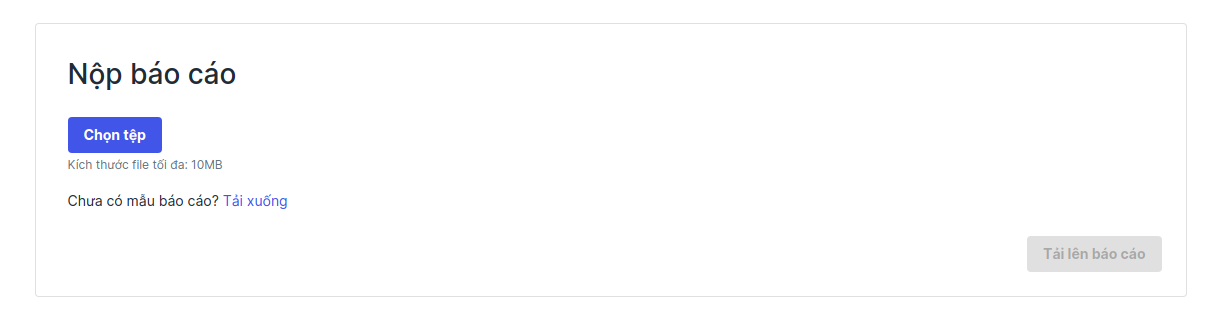
\includegraphics[width=\linewidth]{./images/image41.png}
	\caption{Luồng \emph{Sinh viên nộp báo cáo}: Truy cập phần nộp báo cáo}
	\label{fig:student_internship_info}
\end{figure}

\begin{figure}[]
	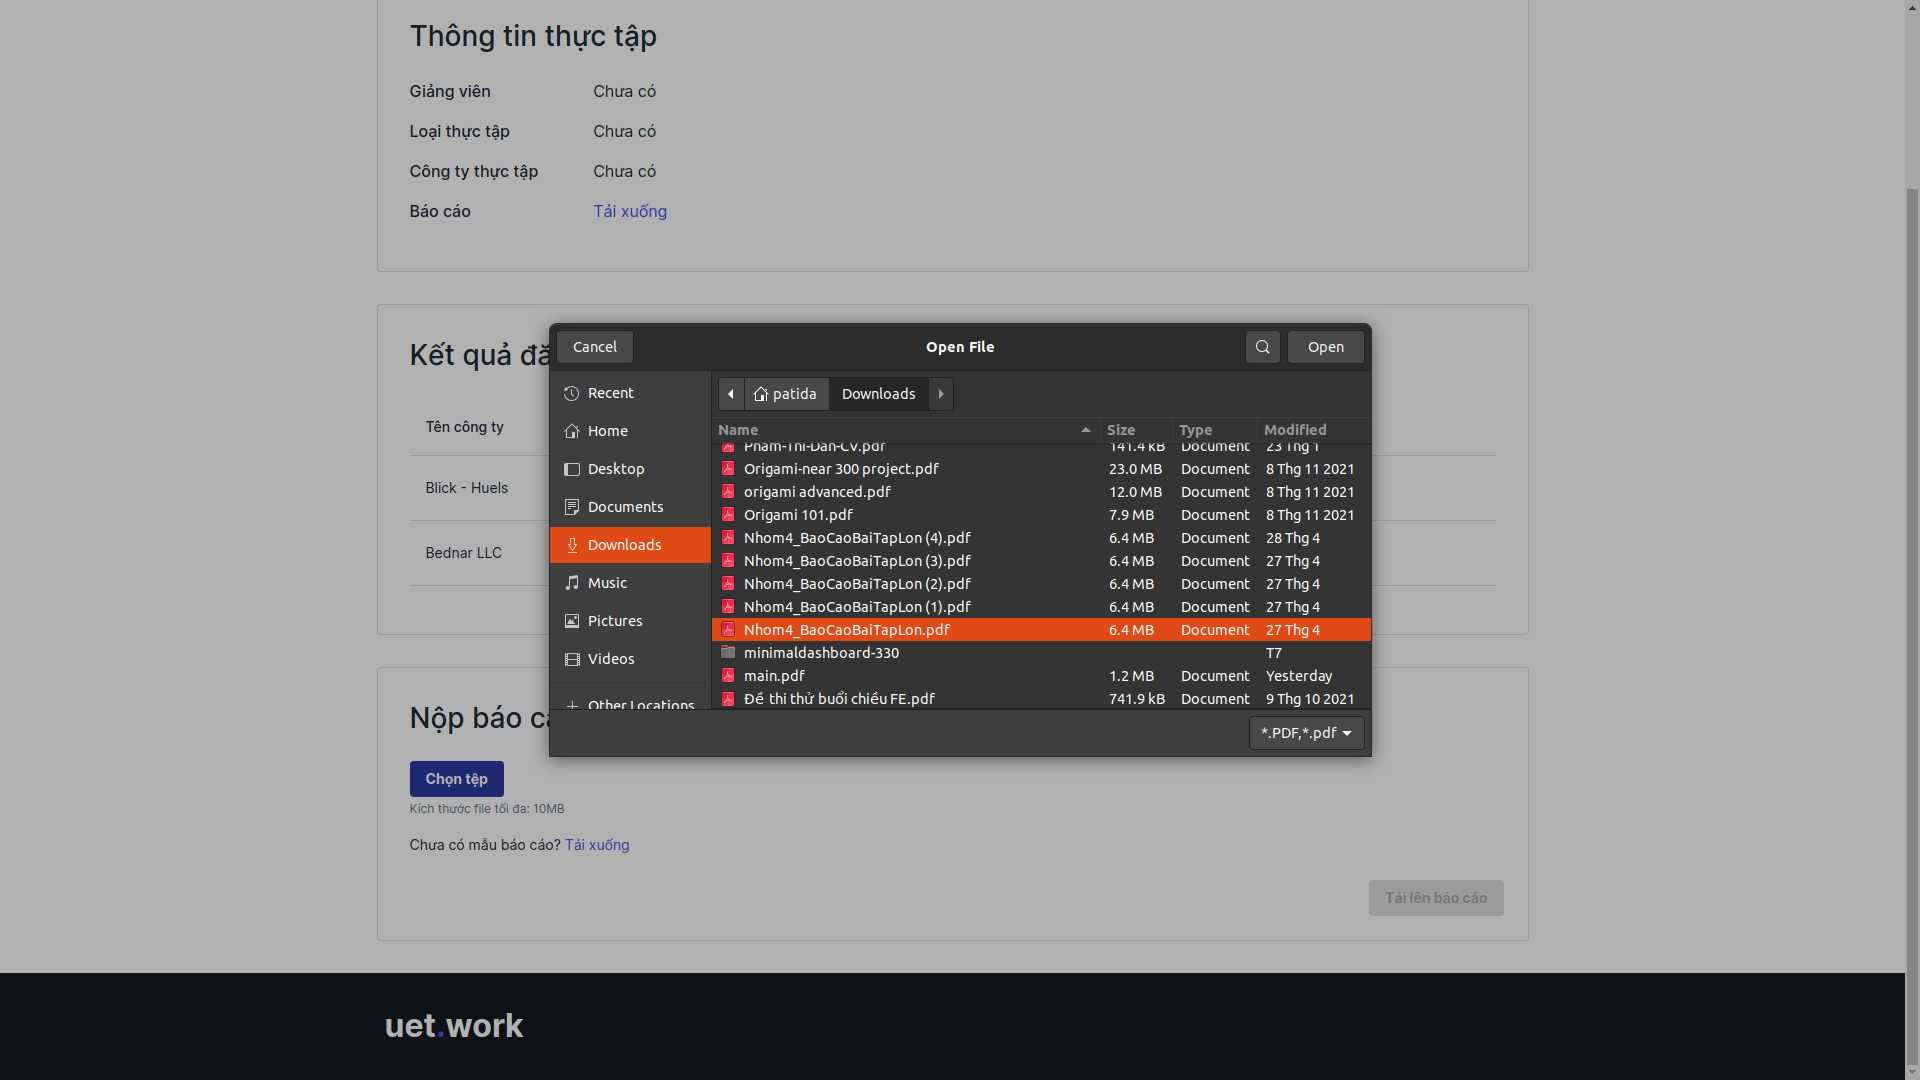
\includegraphics[width=\linewidth]{./images/image42.png}
	\caption{Luồng \emph{Sinh viên nộp báo cáo}: Chọn tệp}
	\label{fig:student_choose_file}
\end{figure}

\begin{figure}[]
	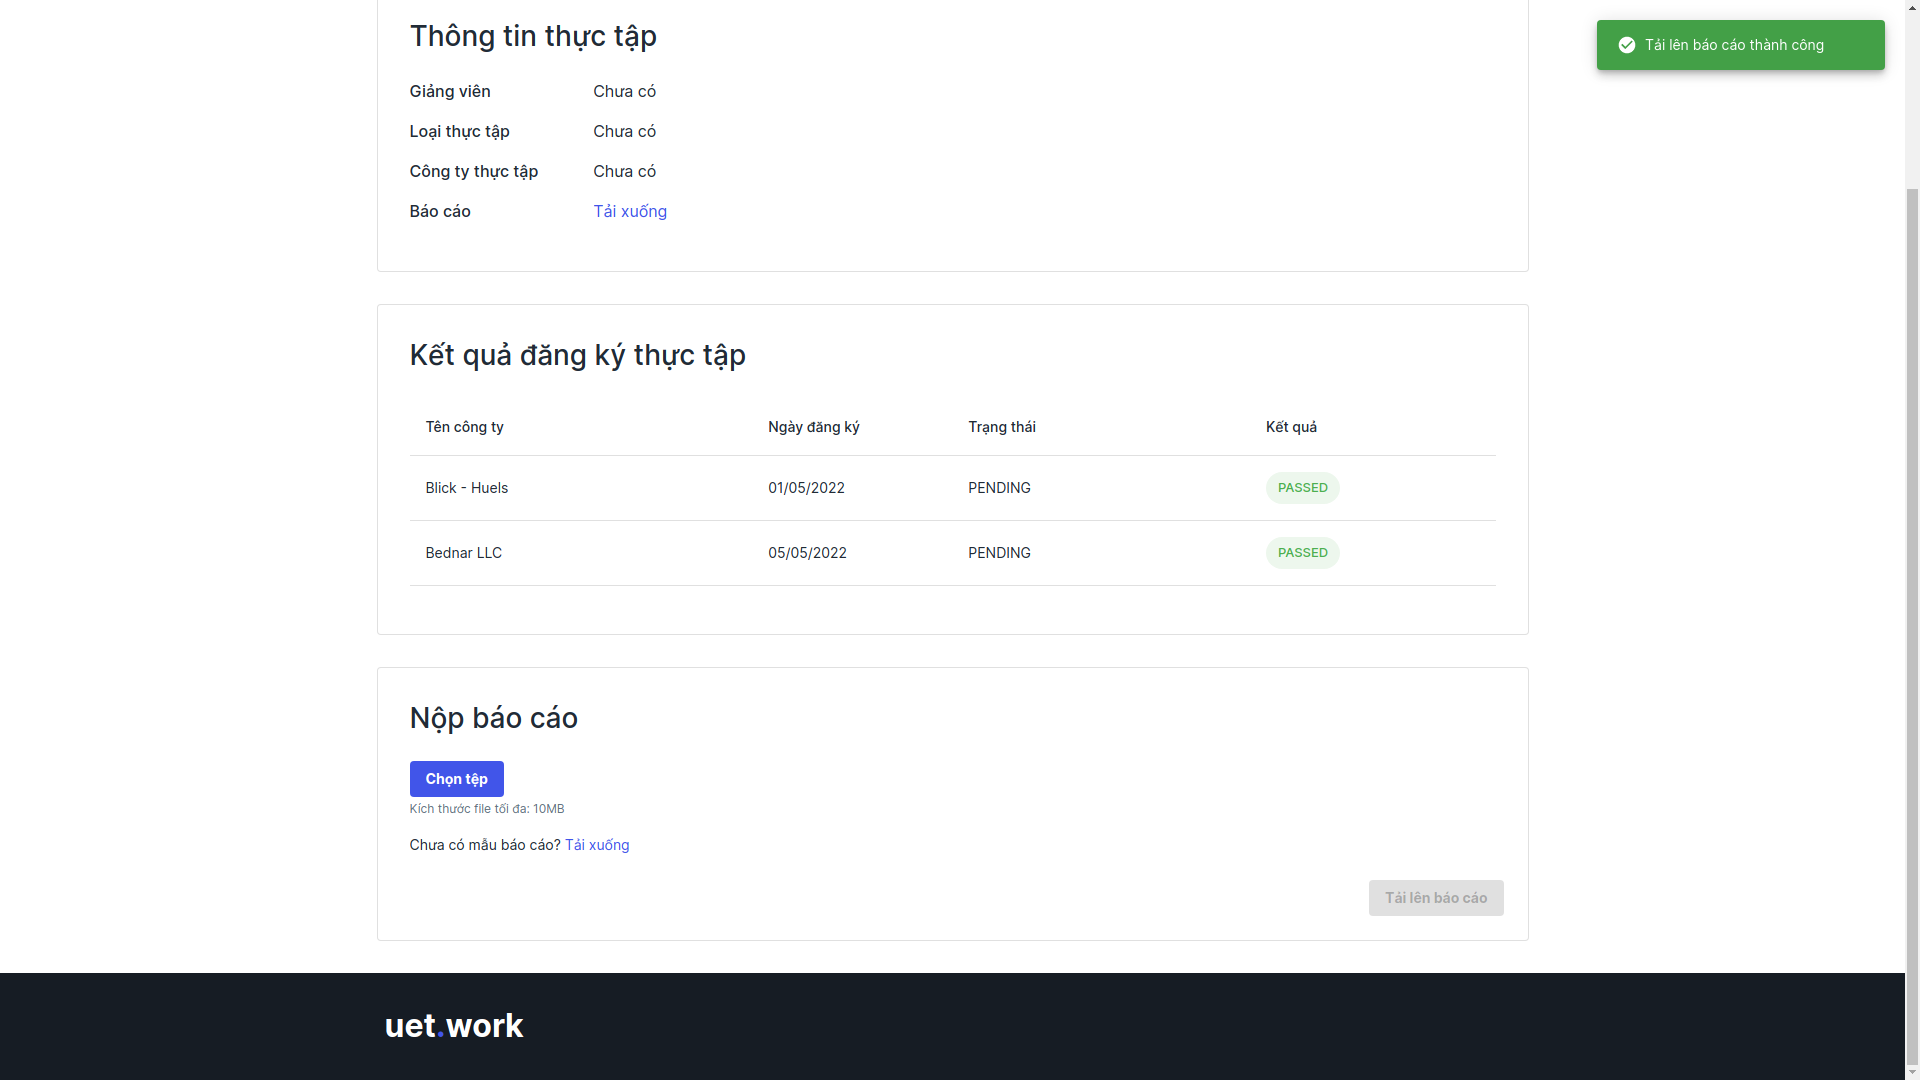
\includegraphics[width=\linewidth]{./images/image43.png}
	\caption{Luồng \emph{Sinh viên nộp báo cáo}: Tải lên báo cáo}
	\label{fig:student_upload_report}
\end{figure}

\paragraph*{Sinh viên xem thông tin cá nhân}
Sinh viên truy cập trang thông tin cá nhân. Tại đây sinh viên có thể sửa thông tin cá nhân, đổi mật khẩu.

Hình \ref{fig:view_info_page} mô tả màn hình trang thông tin cá nhân.

\begin{figure}[]
	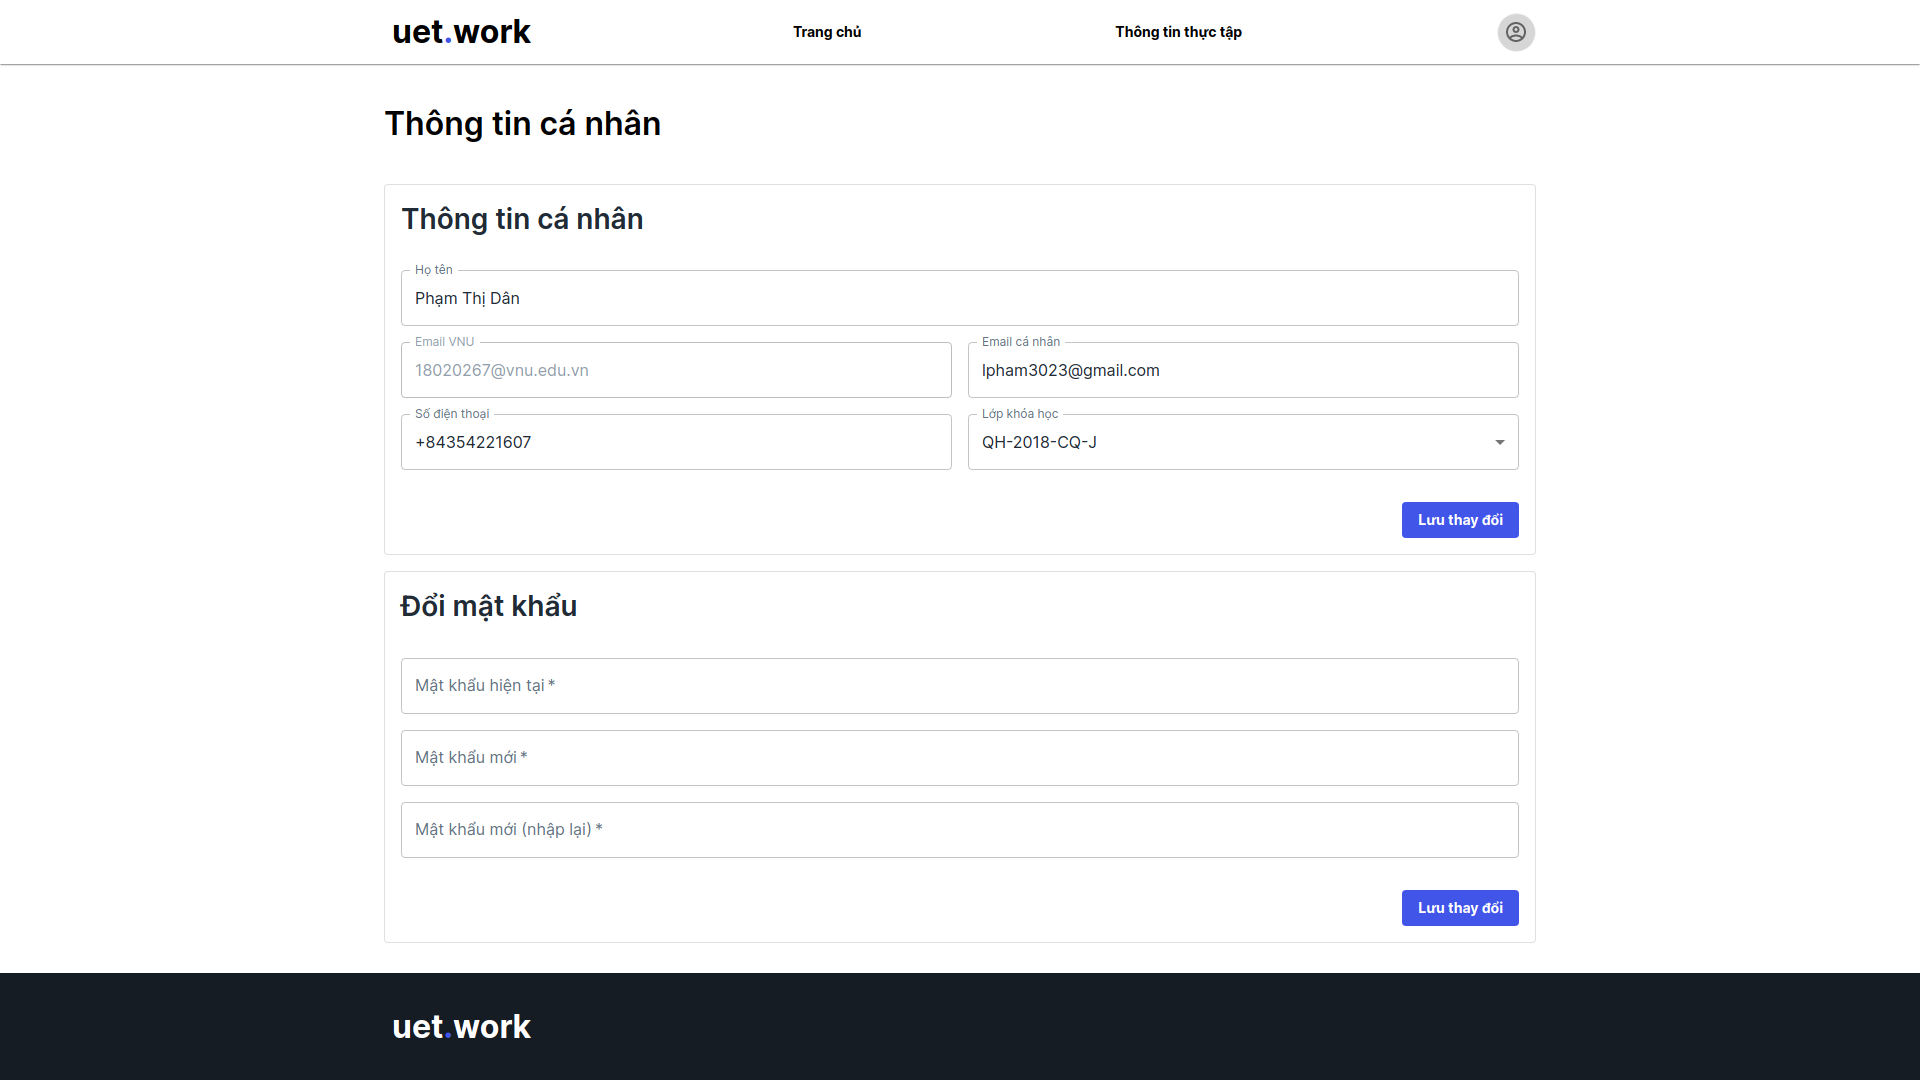
\includegraphics[width=\linewidth]{./images/image44.png}
	\caption{Luồng \emph{Sinh viên xem thông tin cá nhân}}
	\label{fig:view_info_page}
\end{figure}

\paragraph*{Sinh viên thay đổi thông tin cá nhân}

\begin{itemize}
	\item Hình \ref{fig:student_access_info}: Sinh viên truy cập phần thông tin cá nhân.
	\item Hình \ref{fig:student_edit_info}: Sinh viên sửa thông tin cá nhân, đổi mật khẩu.
\end{itemize}

\begin{figure}[]
	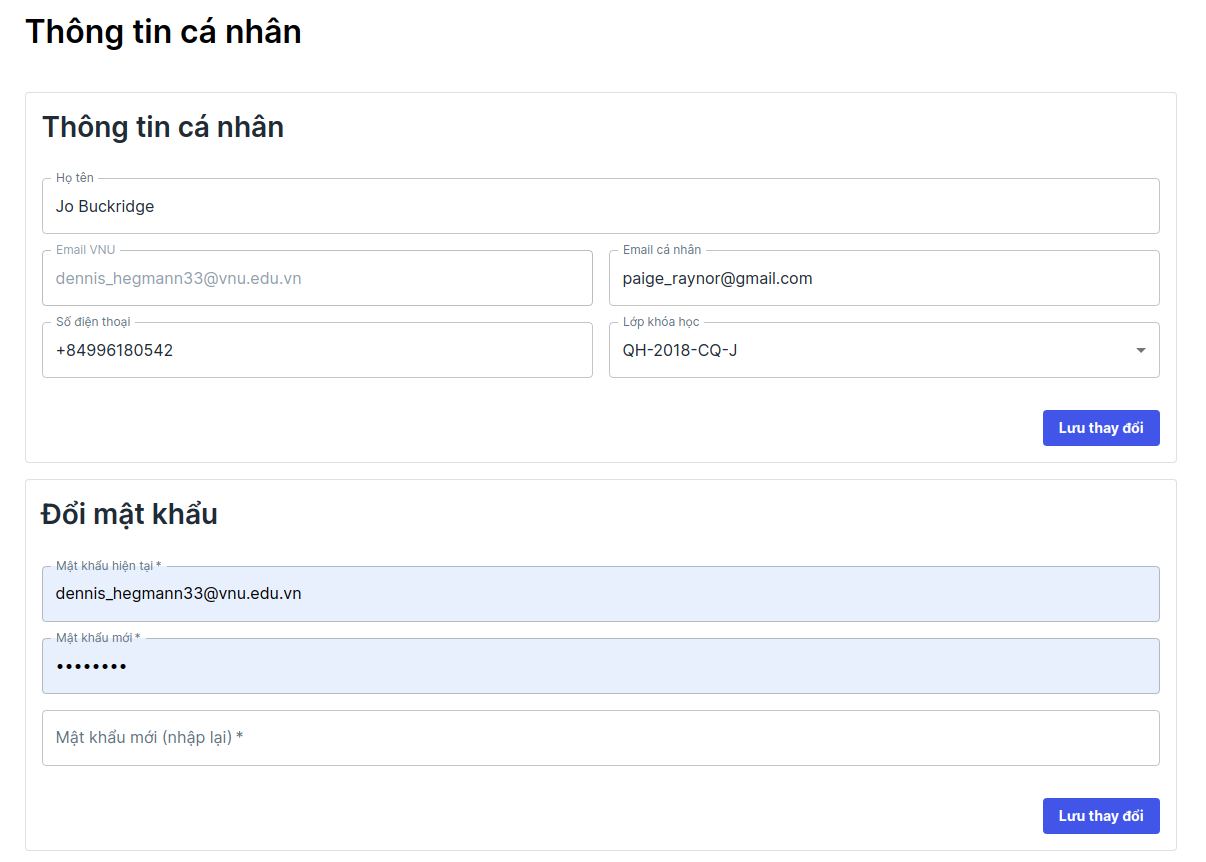
\includegraphics[width=\linewidth]{./images/image45.png}
	\caption{Luồng \emph{Sinh viên thay đổi thông tin cá nhân}: Truy cập trang thông tin cá nhân}
	\label{fig:student_access_info}
\end{figure}

\begin{figure}[]
	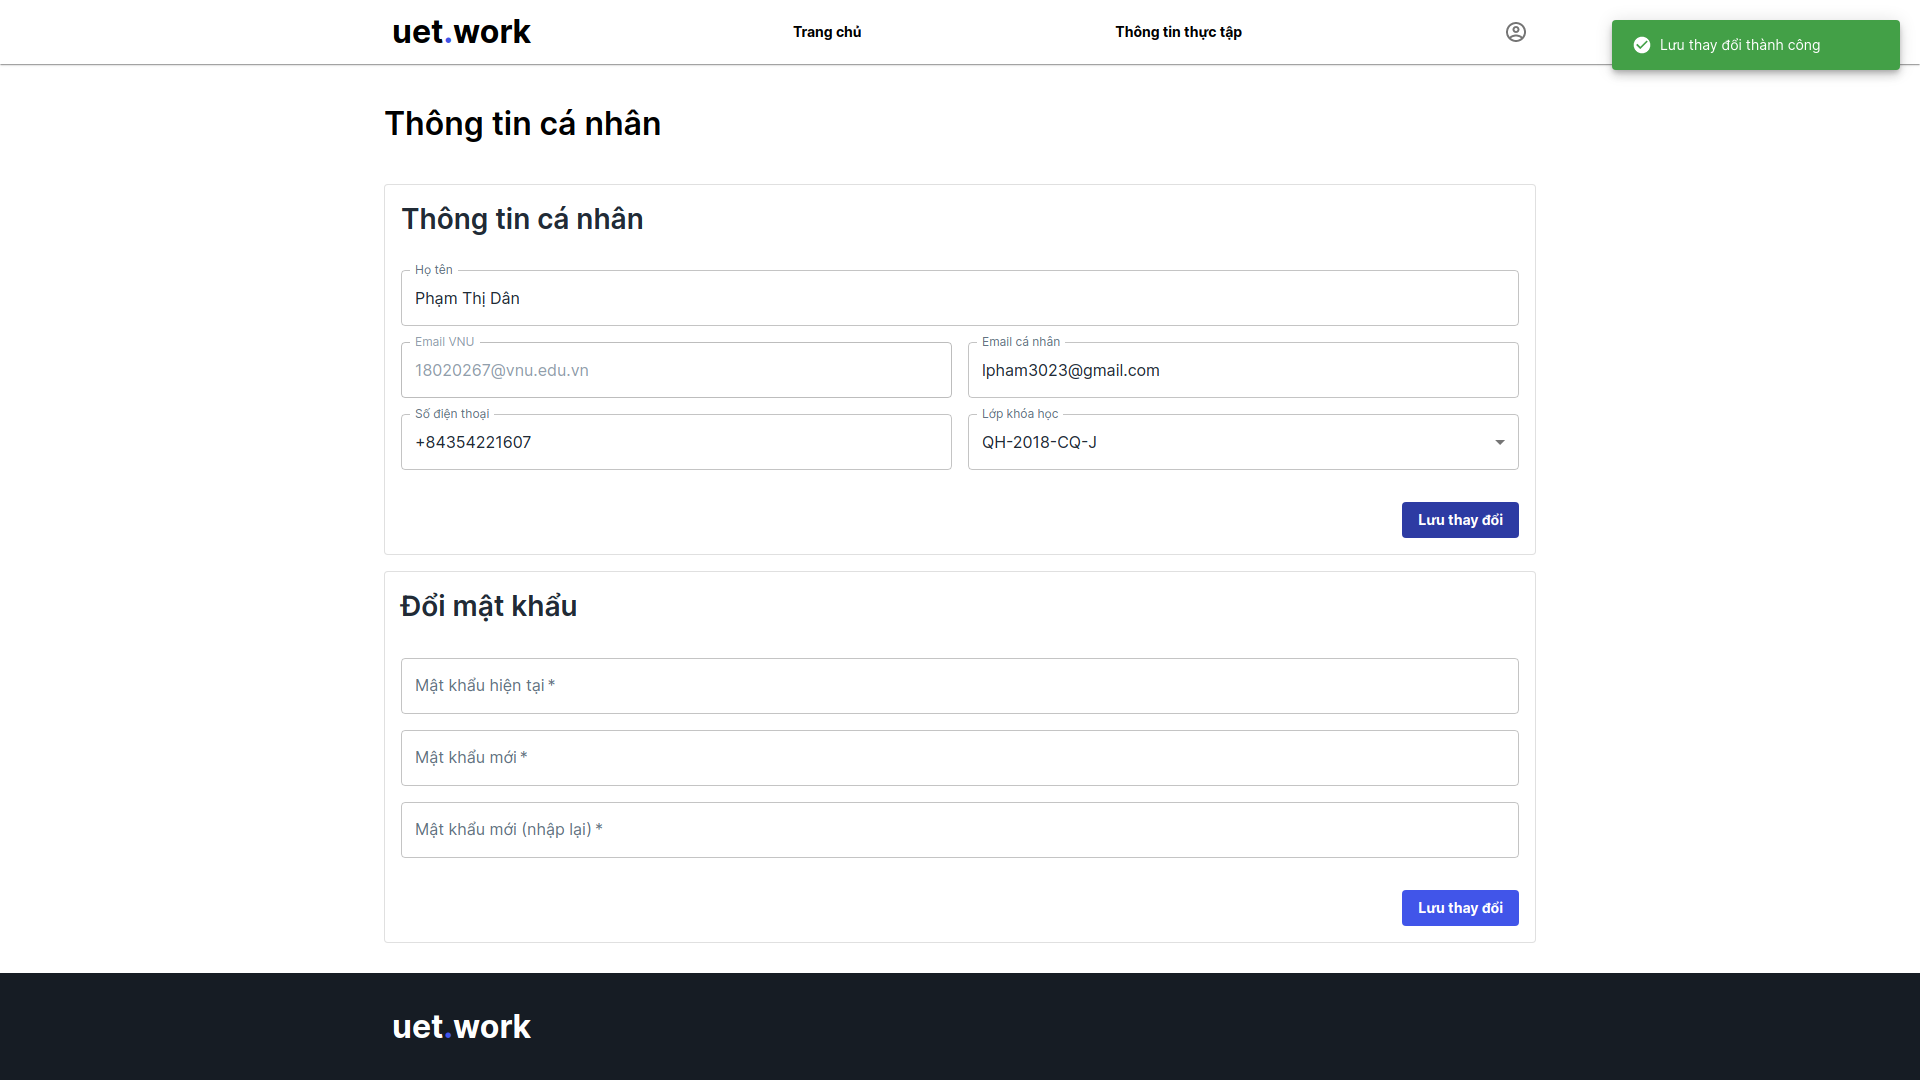
\includegraphics[width=\linewidth]{./images/image46.png}
	\caption{Luồng \emph{Sinh viên thay đổi thông tin cá nhân}: Sinh viên thay đổi thông tin cá nhân}
	\label{fig:student_edit_info}
\end{figure}

\subsubsection{Luồng sử dụng của giảng viên}

\paragraph*{Giảng viên chấm điểm cho sinh viên}

\begin{itemize}
	\item Hình \ref{fig:lecturer_access_students_page}: Giảng viên truy cập trang sinh viên đang hướng dẫn.
	\item Hình \ref{fig:lecturer_score}: Giảng viên chấm điểm cho sinh viên.
\end{itemize}

\begin{figure}[]
	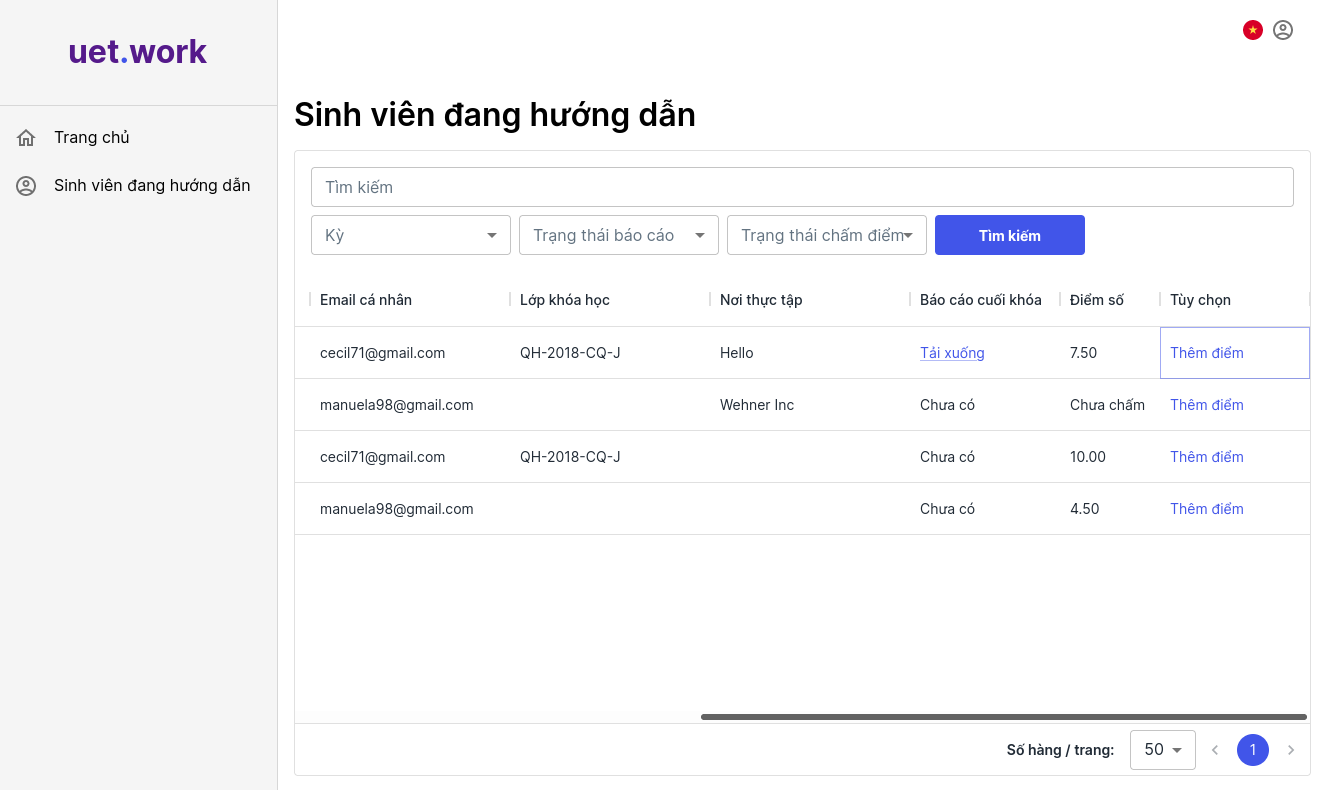
\includegraphics[width=\linewidth]{./images/image64.png}
	\caption{Luồng \emph{Giảng viên chấm điểm cho sinh viên}: Giảng viên truy cập trang sinh viên đang hướng dẫn}
	\label{fig:lecturer_access_students_page}
\end{figure}

\begin{figure}[]
	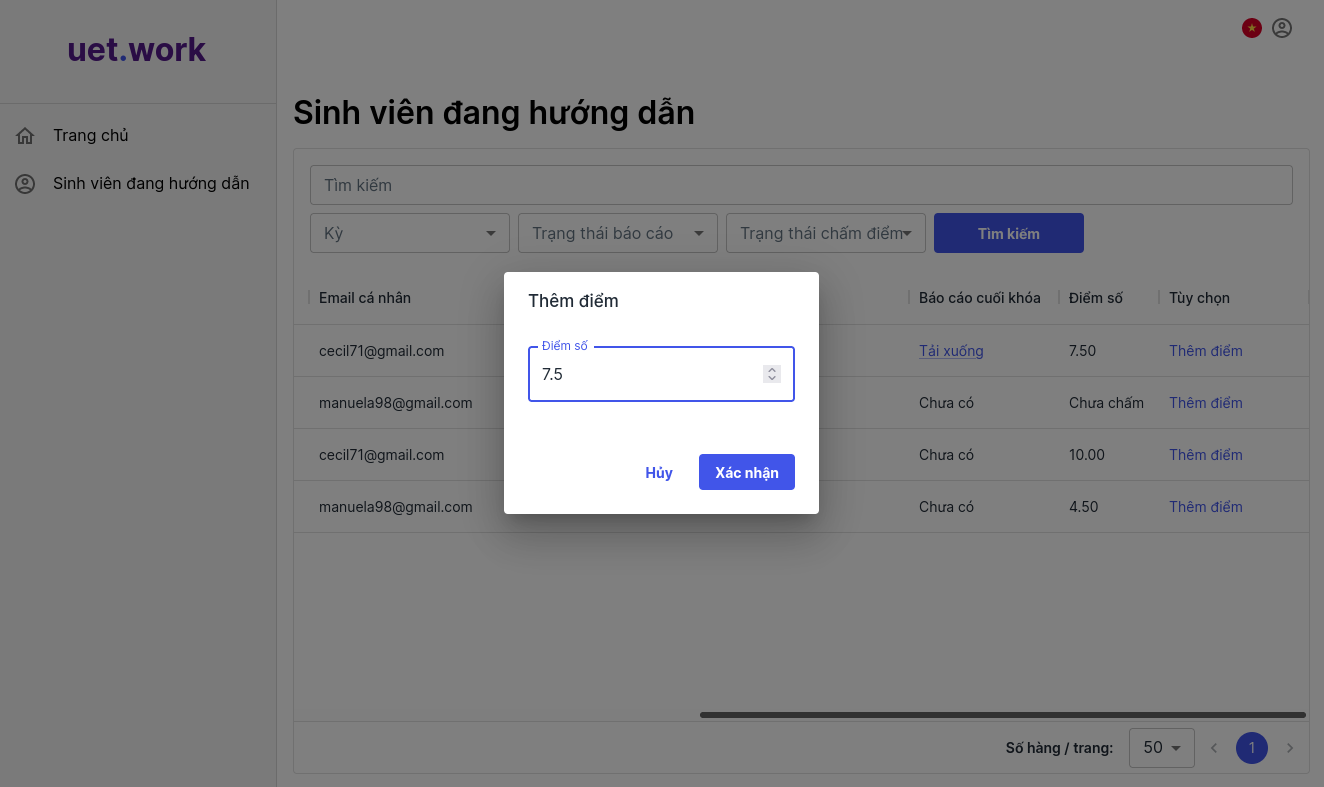
\includegraphics[width=\linewidth]{./images/image65.png}
	\caption{Luồng \emph{Giảng viên chấm điểm cho sinh viên}: Giảng viên chấm điểm cho sinh viên}
	\label{fig:lecturer_score}
\end{figure}

\paragraph*{Giảng viên thay đổi thông tin cá nhân}

\begin{itemize}
	\item Hình \ref{fig:lecturer_access_info_page}: Giảng viên truy cập trang thông tin cá nhân.
	\item Hình \ref{fig:lecturer_edit_info}: Giảng viên thay đổi thông tin cá nhân.
\end{itemize}

\begin{figure}[]
	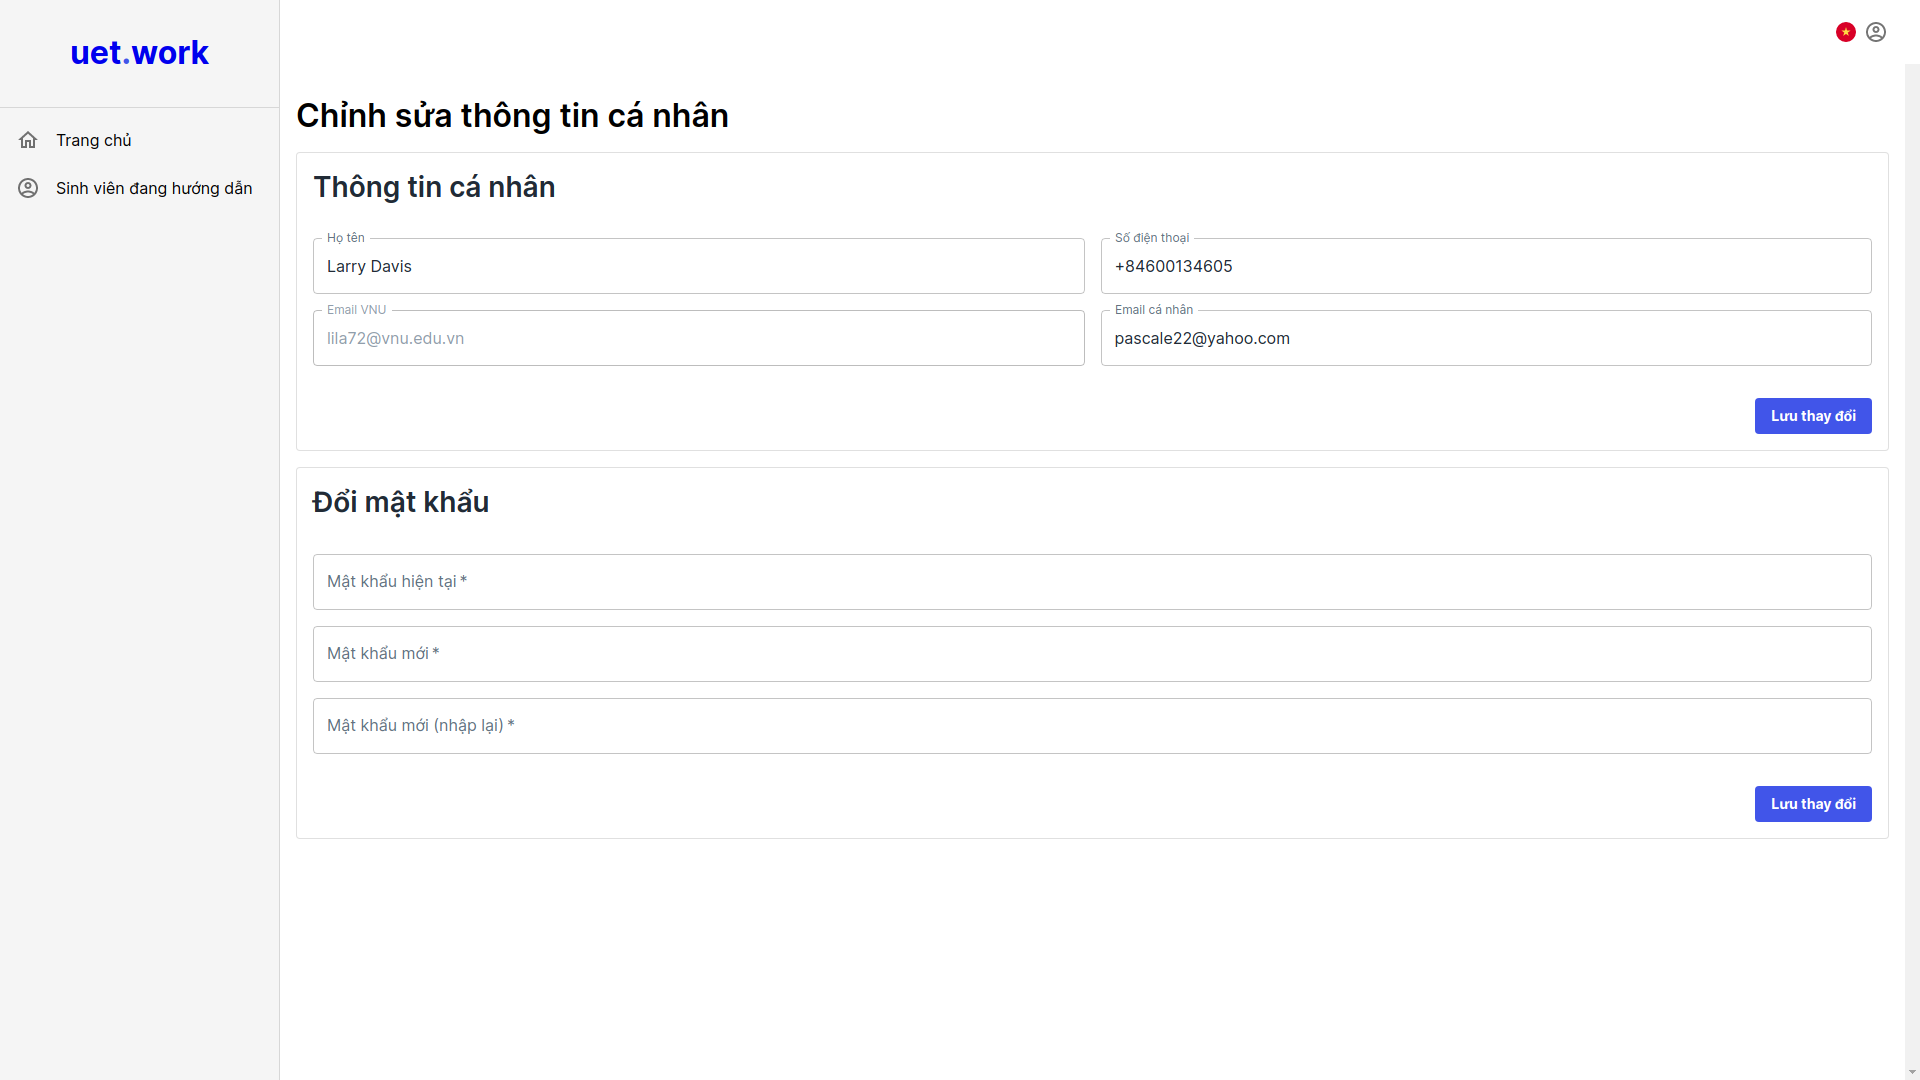
\includegraphics[width=\linewidth]{./images/image51.png}
	\caption{Luồng \emph{Giảng viên thay đổi thông tin cá nhân}: Giảng viên truy cập trang thông tin cá nhân}
	\label{fig:lecturer_access_info_page}
\end{figure}

\begin{figure}[]
	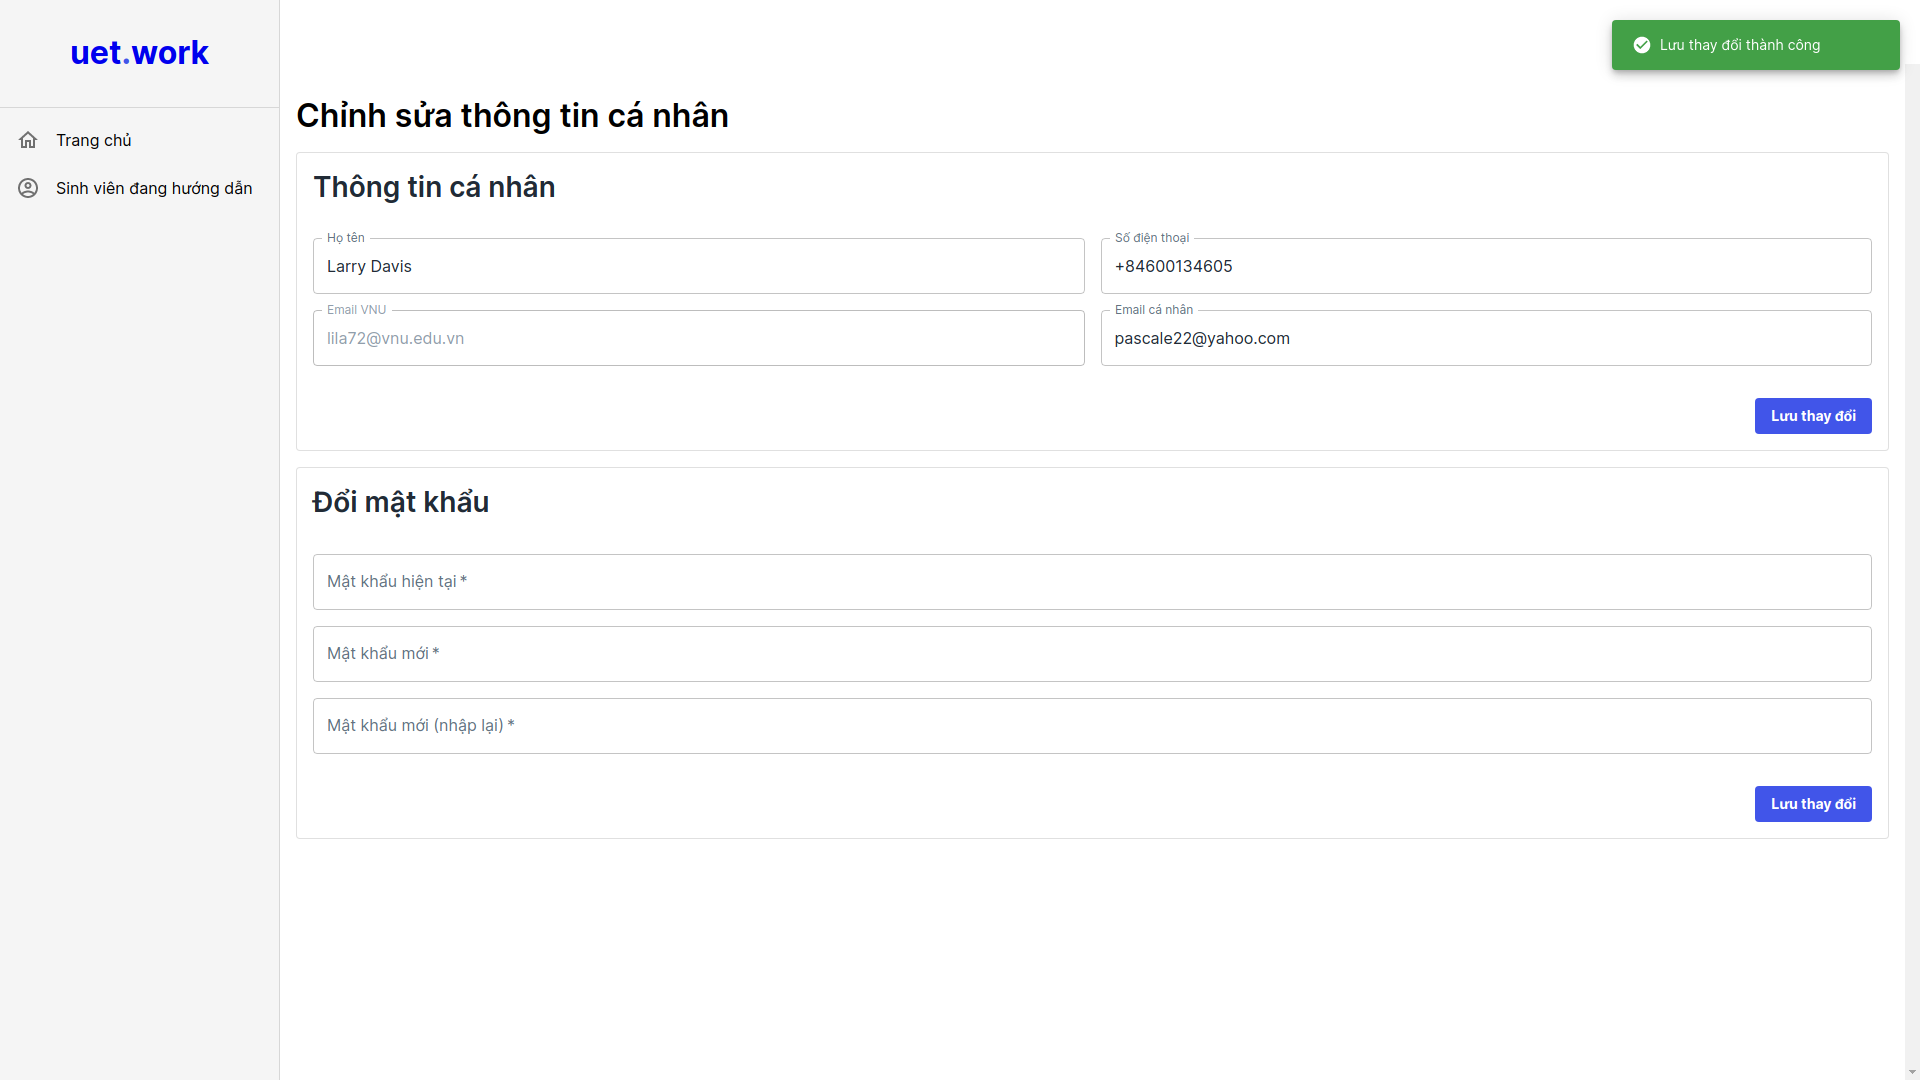
\includegraphics[width=\linewidth]{./images/image52.png}
	\caption{Luồng \emph{Giảng viên thay đổi thông tin cá nhân}: Giảng viên thay đổi thông tin cá nhân}
	\label{fig:lecturer_edit_info}
\end{figure}

\subsubsection{Luồng sử dụng của đối tác}

\paragraph*{Đối tác Chấp nhận / Từ chối yêu cầu thực tập}

\begin{itemize}
	\item Hình \ref{fig:partner_list_requests_page}: Đối tác truy cập danh sách Yêu cầu đăng ký thực tập.
	\item Hình \ref{fig:partner_select_students_approve}: Đối tác chọn sinh viên và chọn Chấp nhận.
	\item Hình \ref{fig:partner_select_students_reject}: Đối tác chọn sinh viên và chọn Từ chối.
\end{itemize}

\begin{figure}[]
	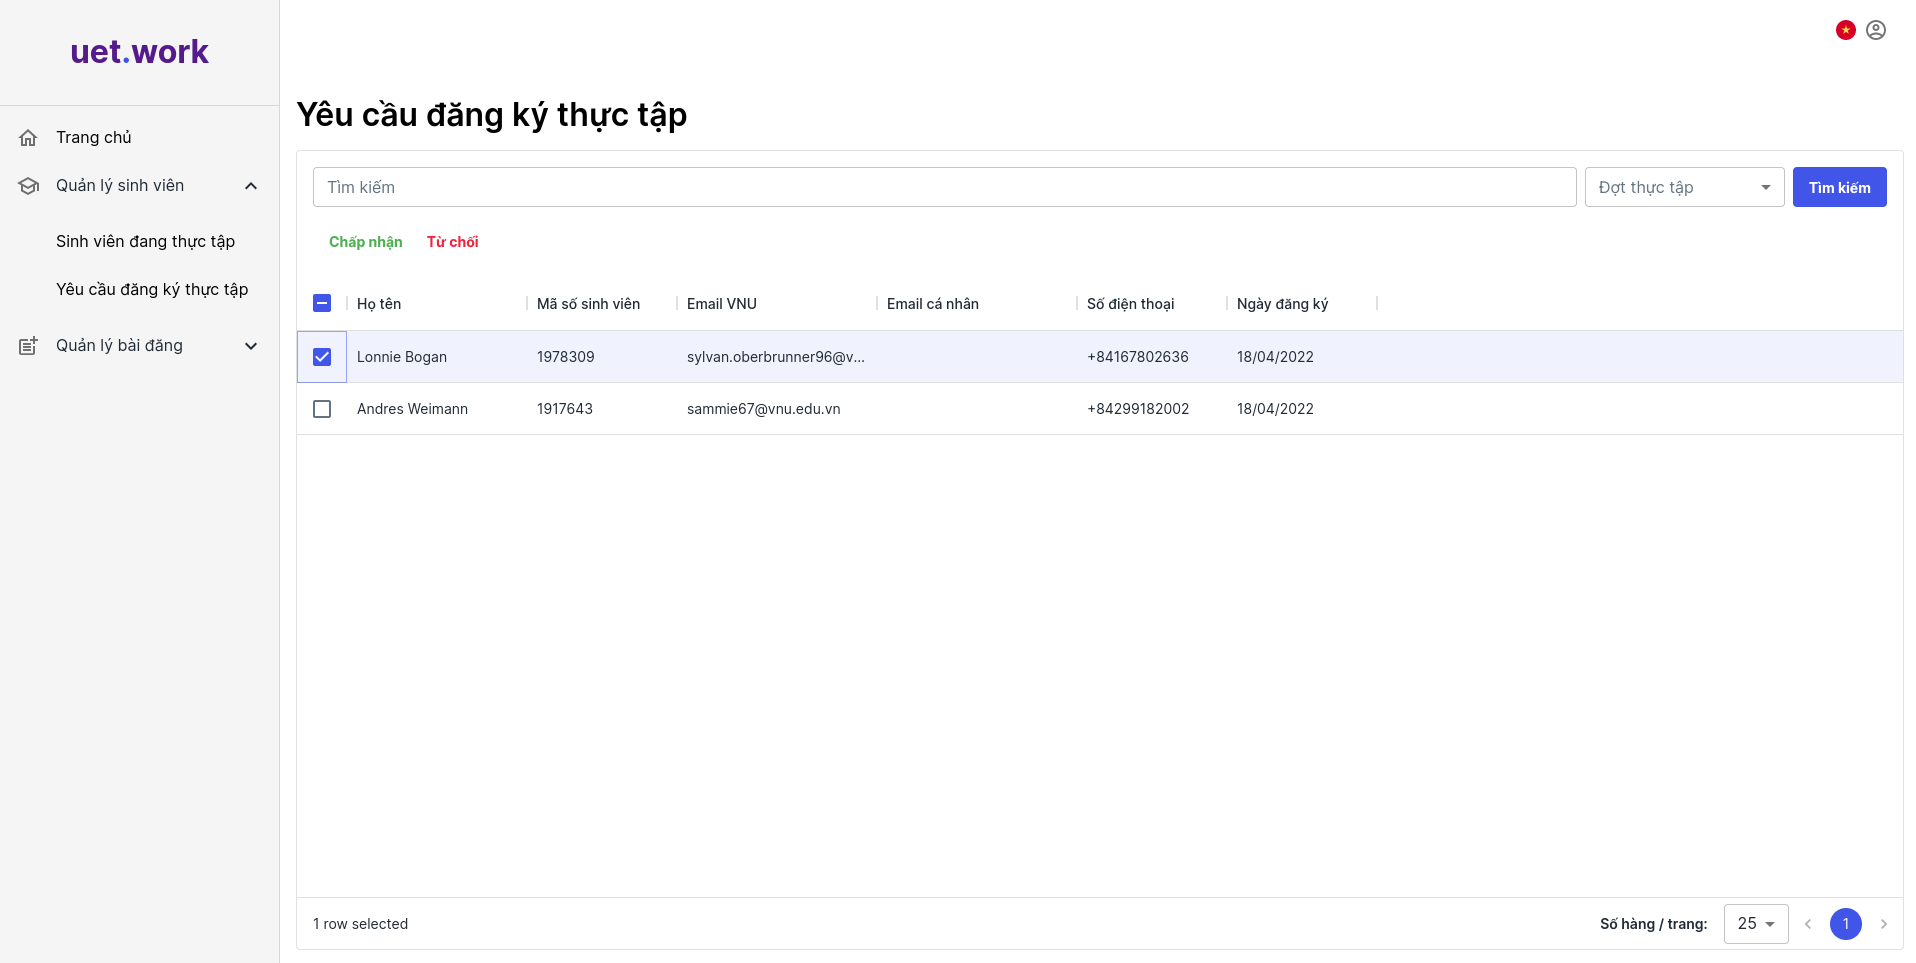
\includegraphics[width=\linewidth]{./images/image29.png}
	\caption{Luồng \emph{Đối tác Chấp nhận / Từ chối yêu cầu thực tập}: truy cập danh sách Yêu cầu đăng ký thực tập}
	\label{fig:partner_list_requests_page}
\end{figure}

\begin{figure}[]
	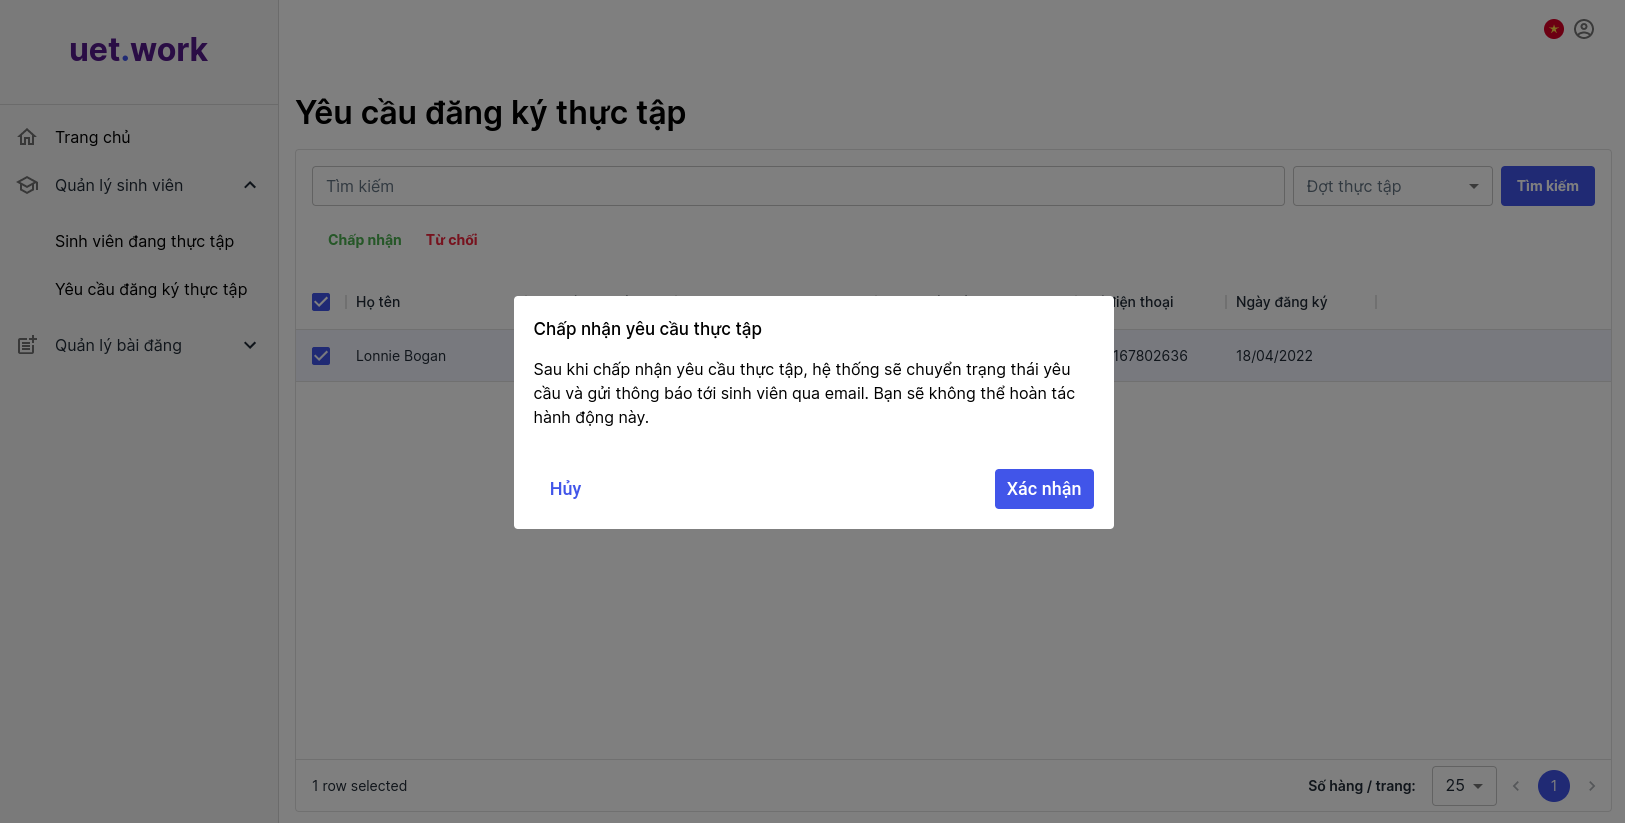
\includegraphics[width=\linewidth]{./images/image66.png}
	\caption{Luồng \emph{Đối tác chấp nhận / Từ chối yêu cầu thực tập}: chọn sinh viên và chọn Chấp nhận}
	\label{fig:partner_select_students_approve}
\end{figure}

\begin{figure}[]
	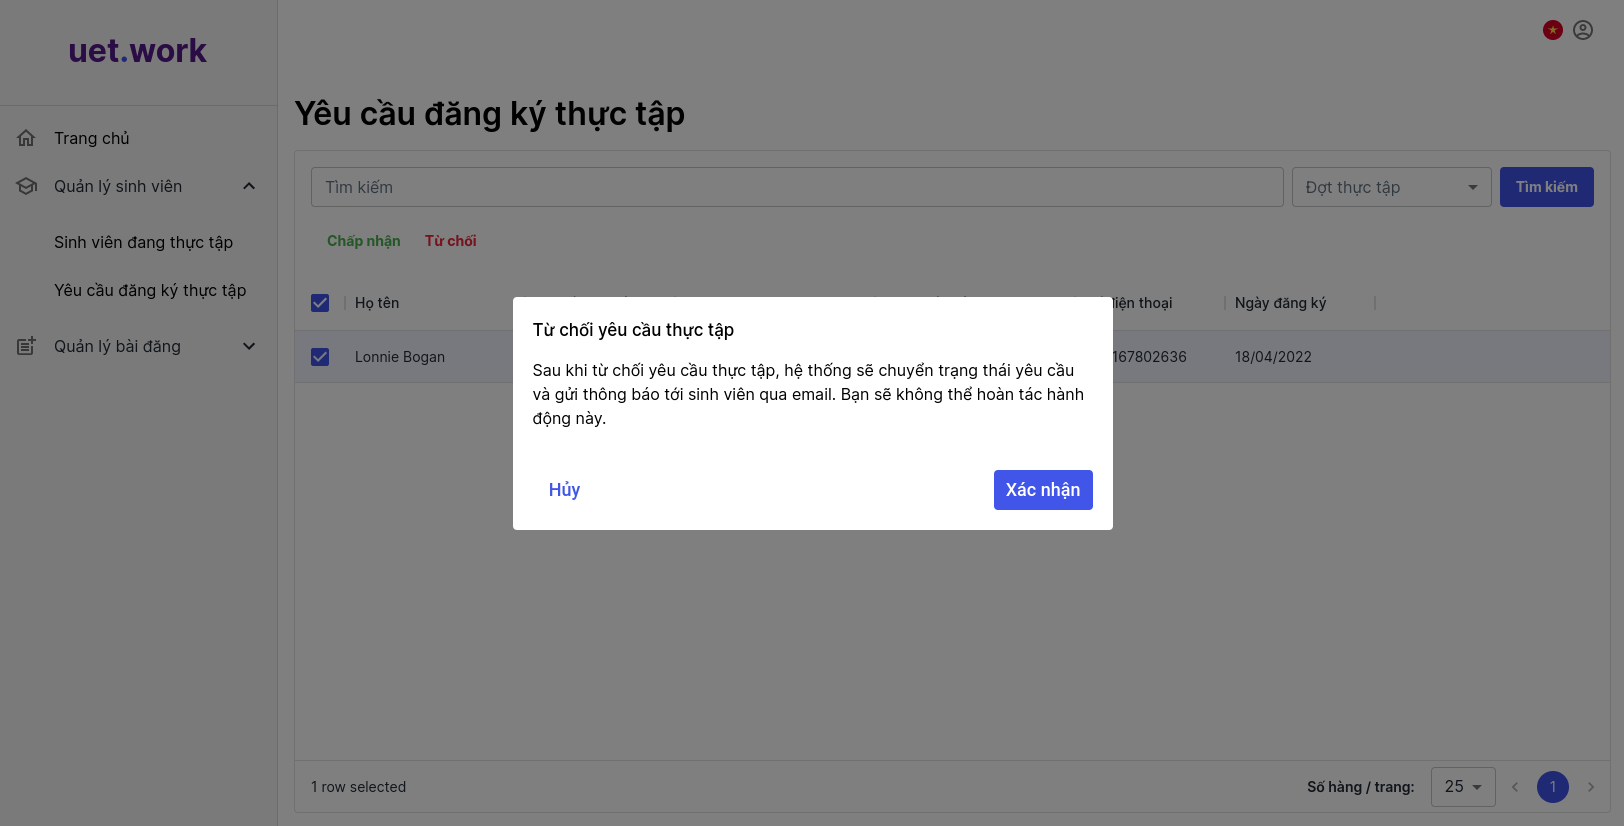
\includegraphics[width=\linewidth]{./images/image67.png}
	\caption{Luồng \emph{Đối tác Chấp nhận / Từ chối yêu cầu thực tập}: chọn sinh viên và chọn Từ chối}
	\label{fig:partner_select_students_reject}
\end{figure}

\paragraph*{Đối tác xem danh sách sinh viên đang thực tập}

Đối tác truy cập trang Sinh viên đang thực tập. Tại đây, đối tác có thể tìm kiếm, sắp xếp và lọc danh sách theo kỳ thực tập.

Hình \ref{fig:partner_view_list_working_students_page} mô tả màn hình danh sách sinh viên đang thực tập.

\begin{figure}[]
	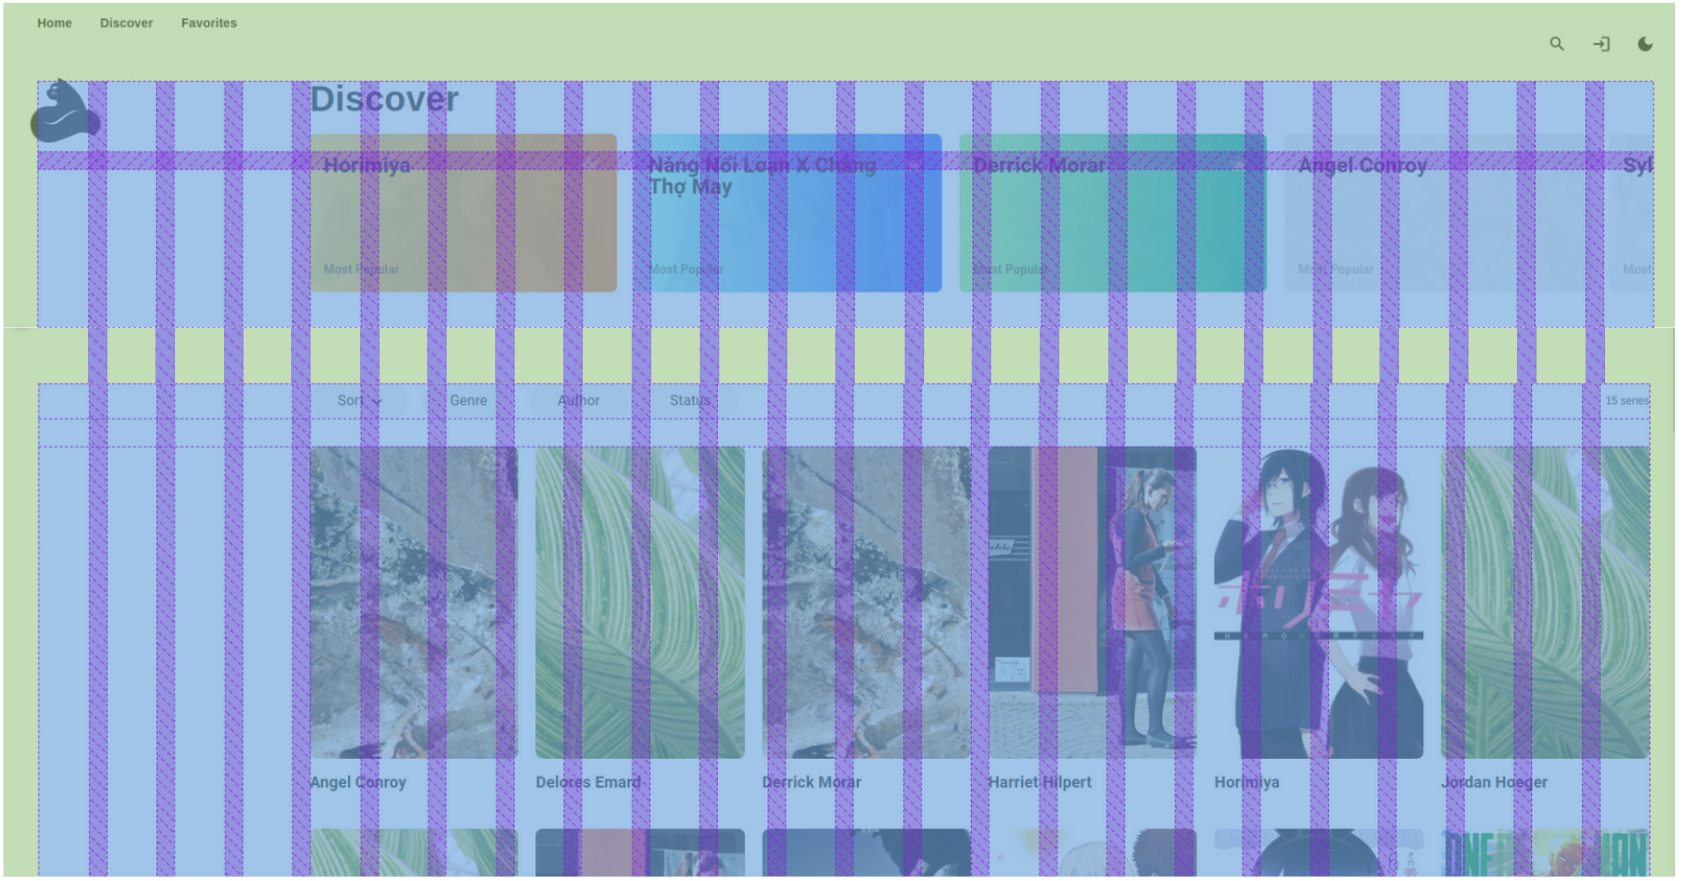
\includegraphics[width=\linewidth]{./images/image9.png}
	\caption{Luồng \emph{Đối tác xem danh sách sinh viên đang thực tập}}
	\label{fig:partner_view_list_working_students_page}
\end{figure}

\paragraph*{Đối tác sửa / thêm liên hệ}

\begin{itemize}
	\item Hình \ref{fig:partner_info_page}: Đối tác truy cập trang thông tin cá nhân.
	\item Hình \ref{fig:partner_upsert_contact}: Đối tác Sửa/Thêm liên hệ.
\end{itemize}

\begin{figure}[]
	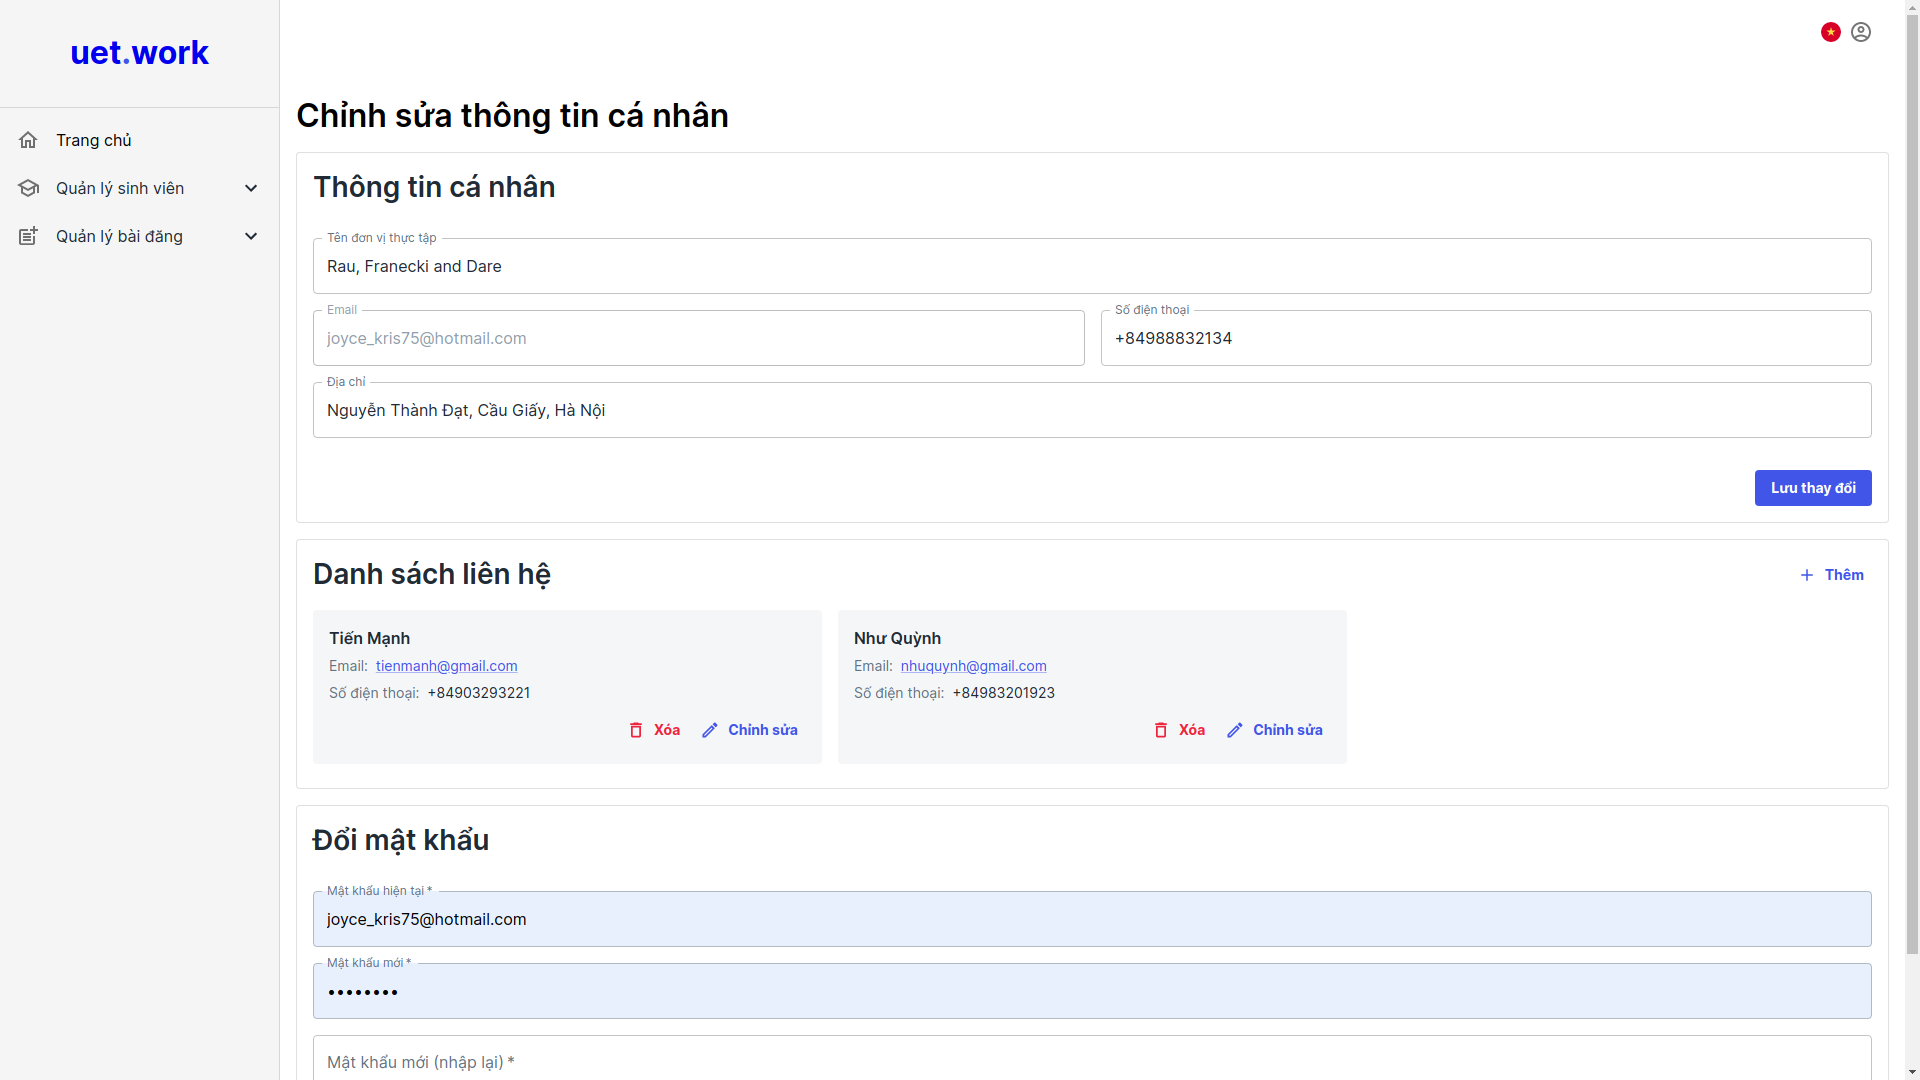
\includegraphics[width=\linewidth]{./images/image48-1.png}
	\caption{Luồng \emph{Đối tác sửa / thêm liên hệ}: Truy cập trang thông tin cá nhân}
	\label{fig:partner_info_page}
\end{figure}

\begin{figure}[]
	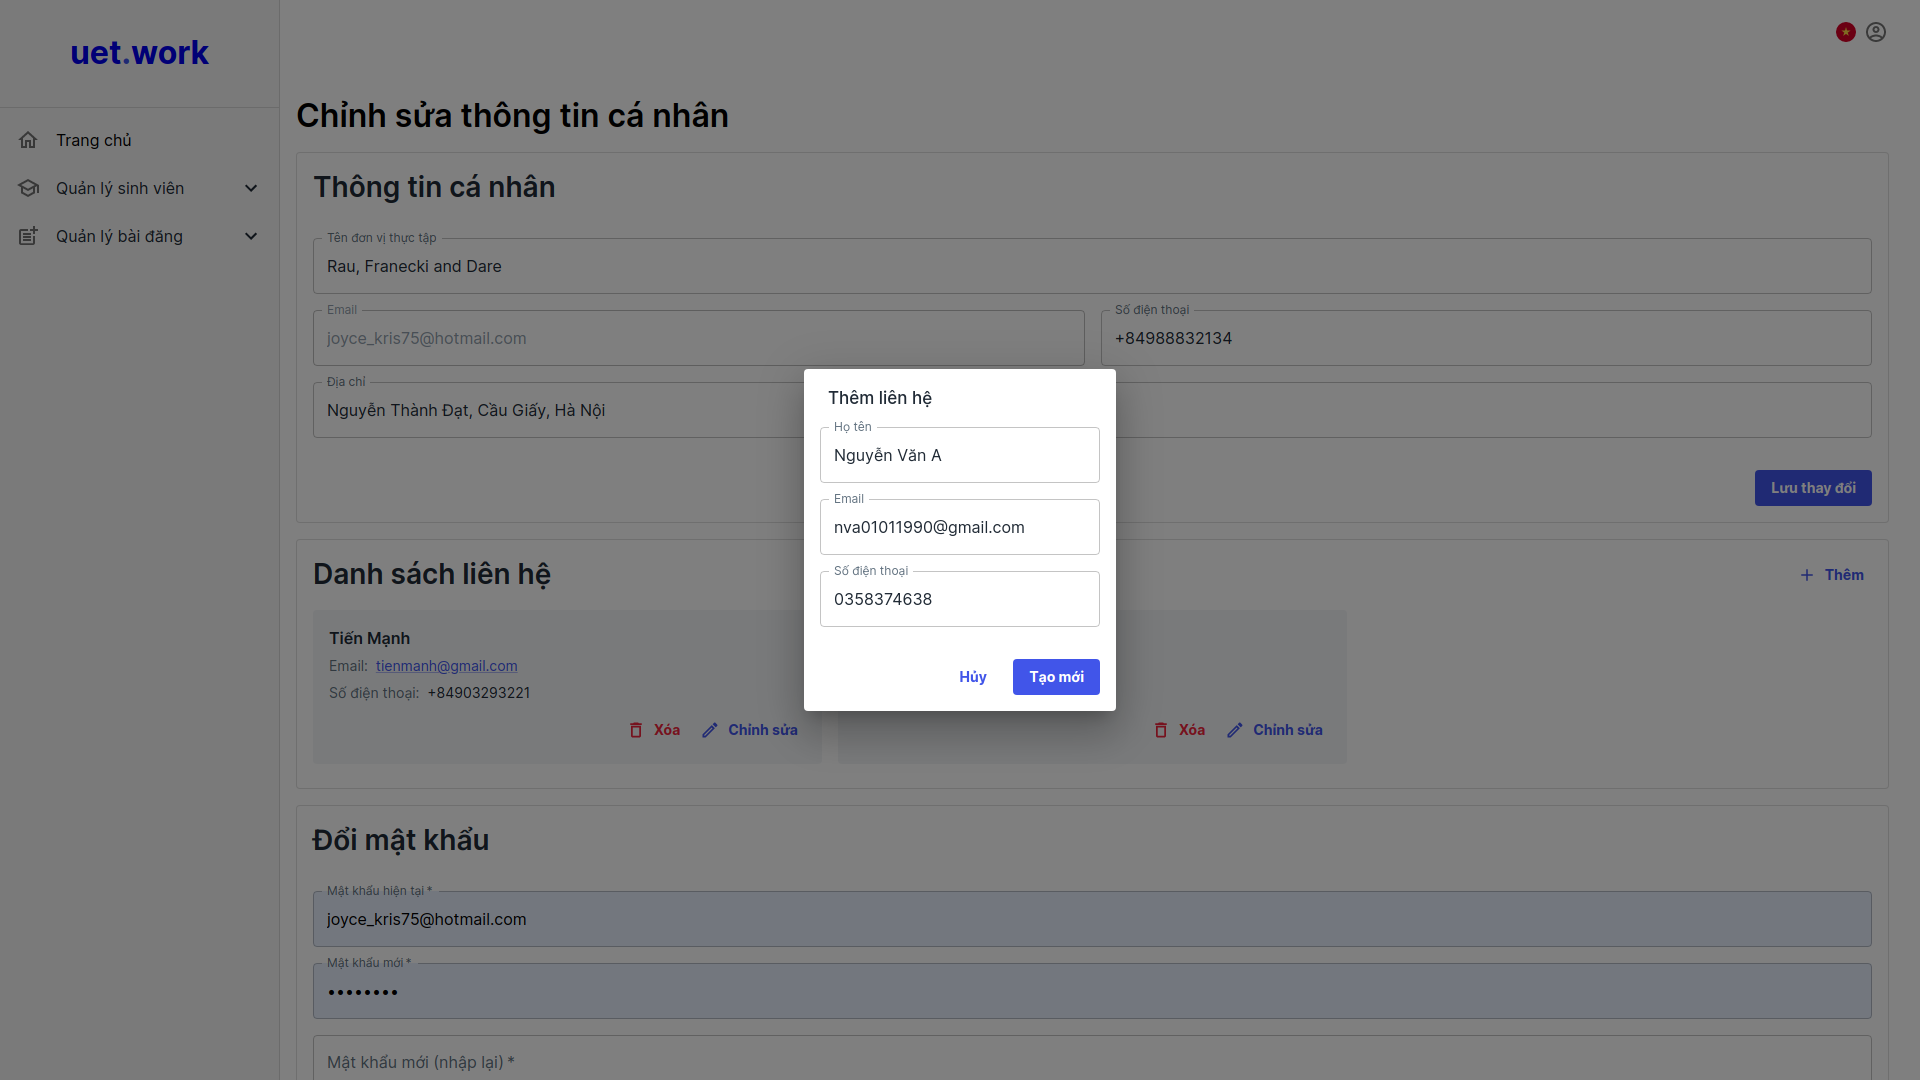
\includegraphics[width=\linewidth]{./images/image48.png}
	\caption{Luồng \emph{Đối tác sửa / thêm liên hệ}: Sửa/Thêm liên hệ}
	\label{fig:partner_upsert_contact}
\end{figure}

\subsubsection{Luồng sử dụng của quản trị viên Khoa}

\paragraph*{Quản trị viên tải xuống danh sách sinh viên đã chốt đơn vị thực tập}

\begin{itemize}
	\item Hình \ref{fig:org_admin_access_list_intern_students}: Quản trị viên truy cập danh sách sinh viên trong kỳ thực tập.
	\item Hình \ref{fig:org_admin_filter_students}: Quản trị viên lọc ra danh sách Sinh viên đã chốt đơn vị thực tập và chọn tùy chọn Xuất ra danh sách sinh viên.
\end{itemize}

\begin{figure}[]
	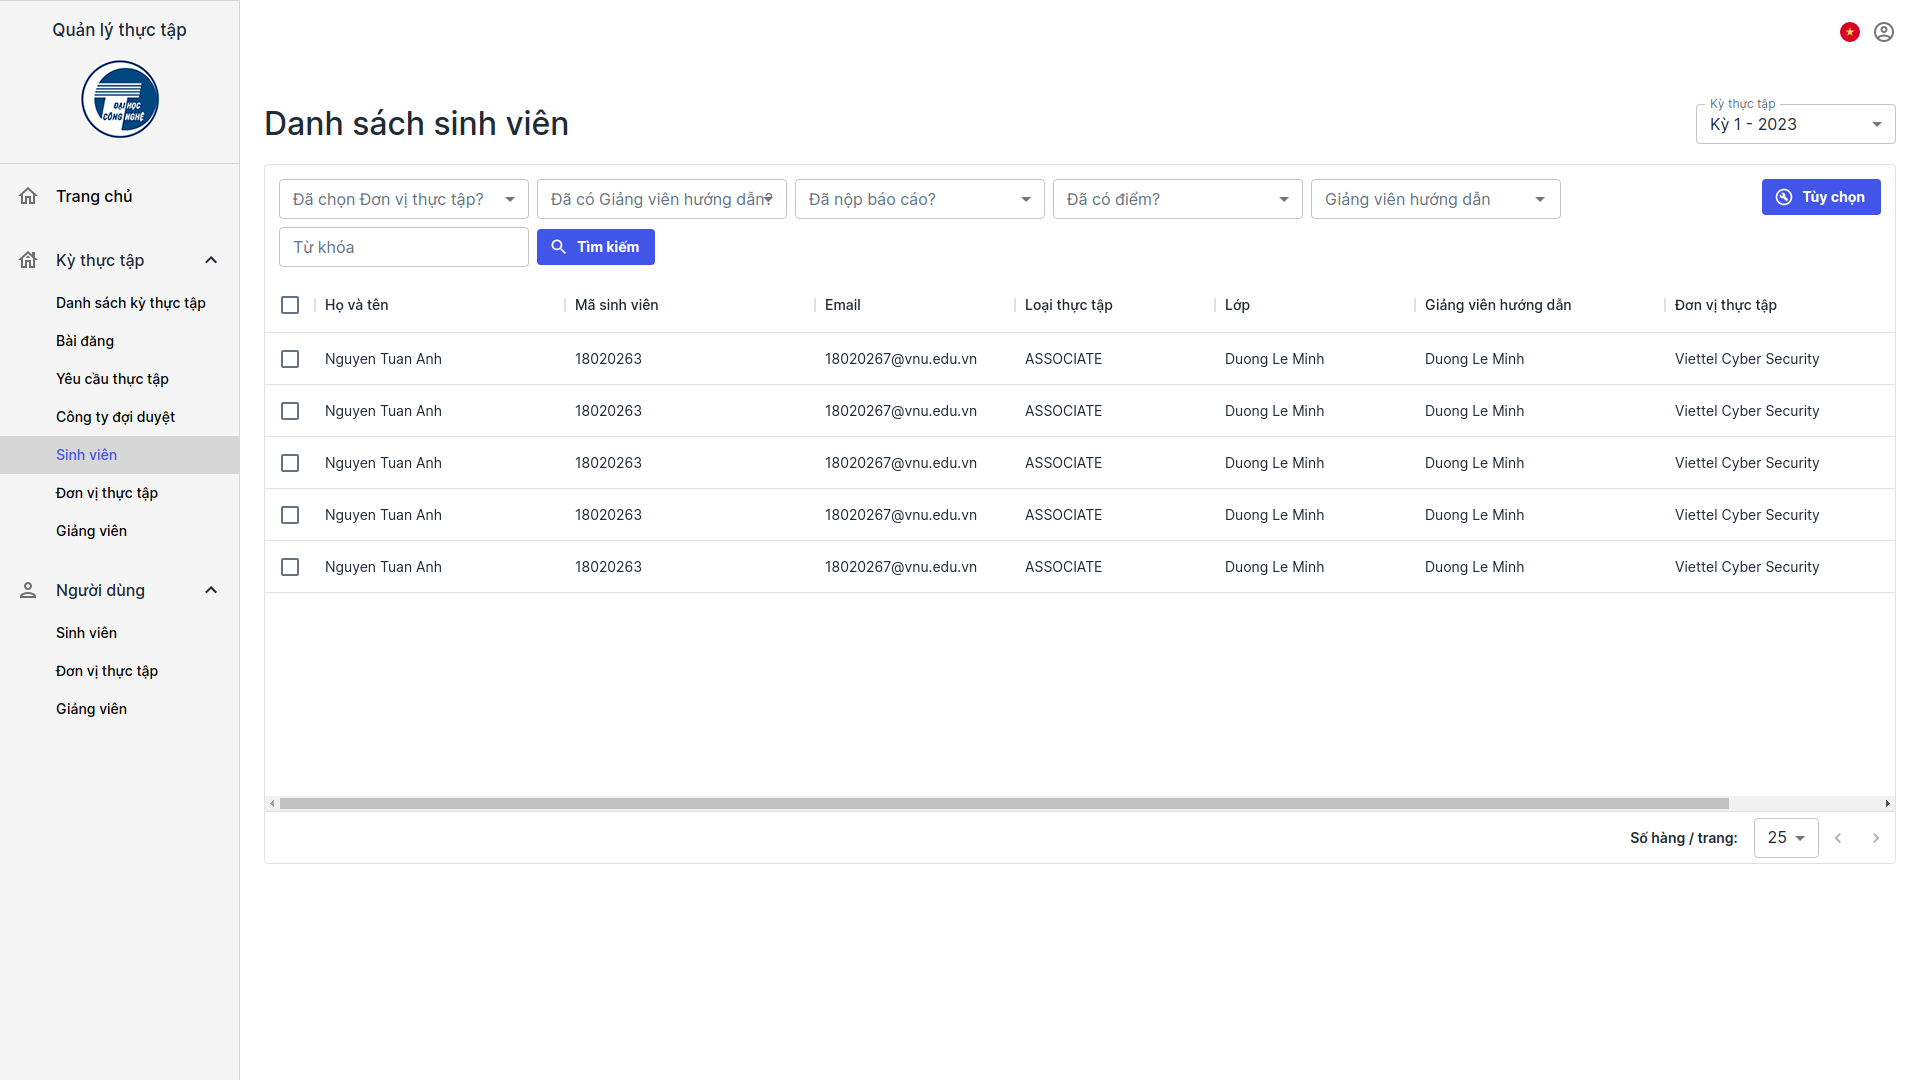
\includegraphics[width=\linewidth]{./images/image75.png}
	\caption{Luồng \emph{Quản trị viên tải xuống danh sách sinh viên đã chốt đơn vị thực tập}: truy cập danh sách sinh viên trong kỳ thực tập}
	\label{fig:org_admin_access_list_intern_students}
\end{figure}

\begin{figure}[]
	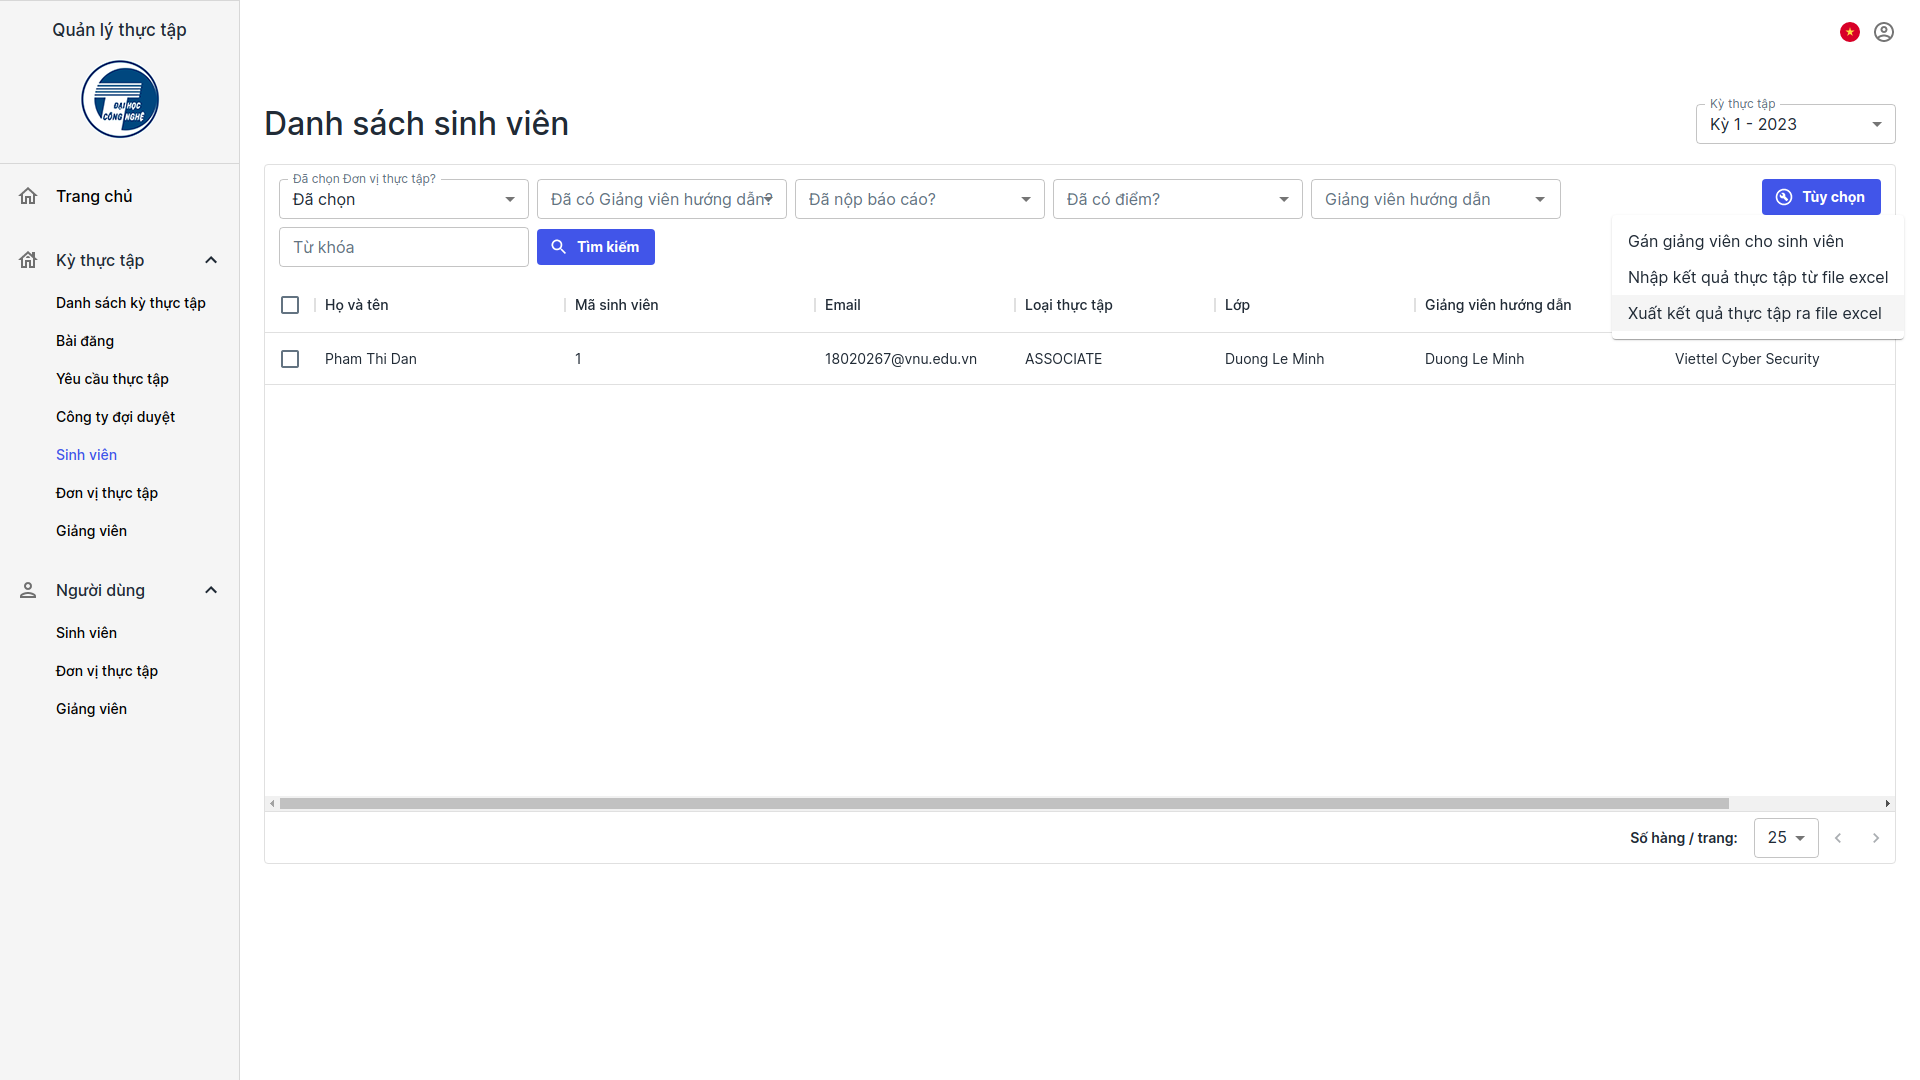
\includegraphics[width=\linewidth]{./images/image74.png}
	\caption{Luồng \emph{Quản trị viên tải xuống danh sách sinh viên đã chốt đơn vị thực tập}: lọc ra danh sách Sinh viên đã chốt đơn vị thực tập và chọn tùy chọn Xuất ra danh sách}
	\label{fig:org_admin_filter_students}
\end{figure}

\paragraph*{Quản trị viên Khoa gán giảng viên cho sinh viên}

\begin{itemize}
	\item Hình \ref{fig:org_admin_access_list_intern_students_1}: Quản trị viên khoa truy cập trang Danh sách sinh viên trong Kỳ thực tập.
	\item Hình \ref{fig:org_admin_select_students}: Quản trị viên Khoa chọn danh sách sinh viên cần gán giảng viên và chọn tùy chọn Gán giảng viên.
	\item Hình \ref{fig:org_admin_select_lecturer}: Quản trị viên Khoa thực hiện chọn giảng viên để gán cho danh sách sinh viên.
	\item Hình \ref{fig:org_admin_assign_success}: Gán giảng viên thành công.
\end{itemize}

\begin{figure}[]
	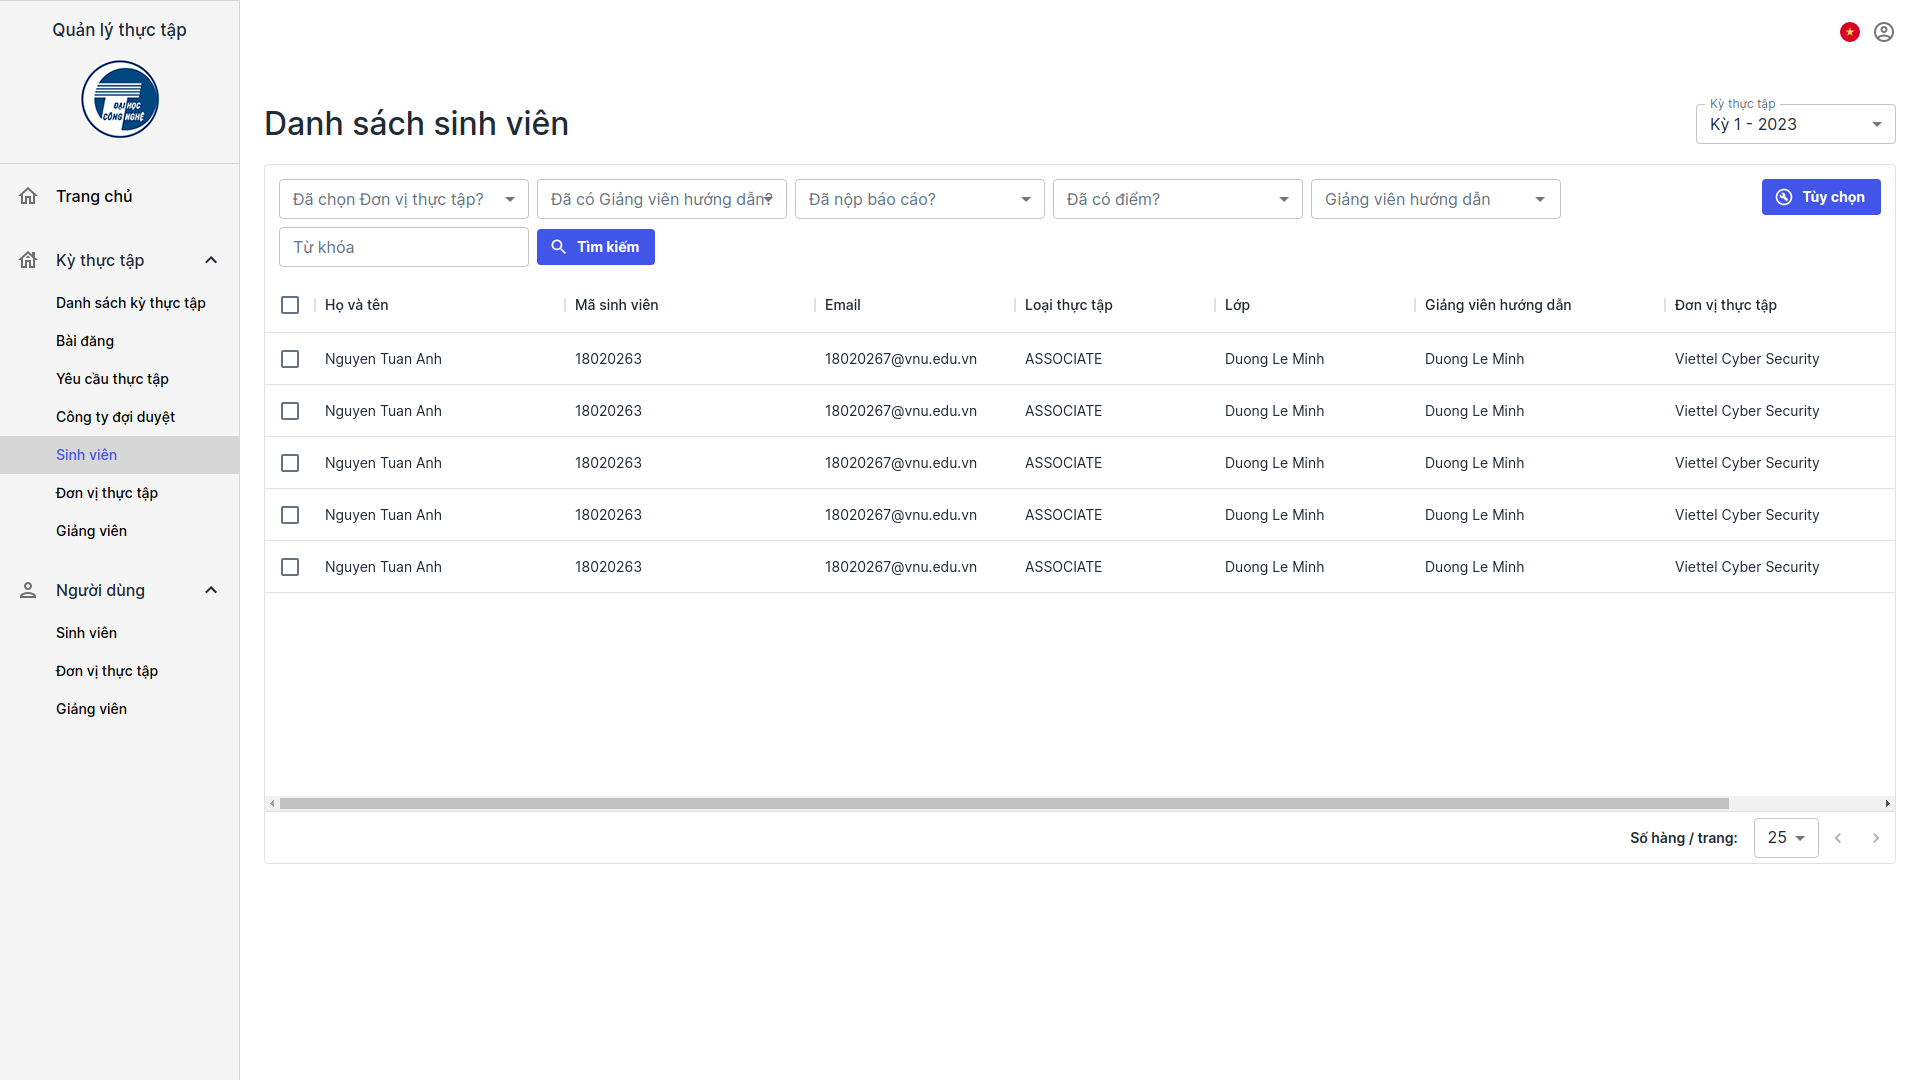
\includegraphics[width=\linewidth]{./images/image75.png}
	\caption{Luồng \emph{Quản trị viên Khoa gán giảng viên cho sinh viên}: truy cập danh sách sinh viên trong kỳ thực tập}
	\label{fig:org_admin_access_list_intern_students_1}
\end{figure}

\begin{figure}[]
	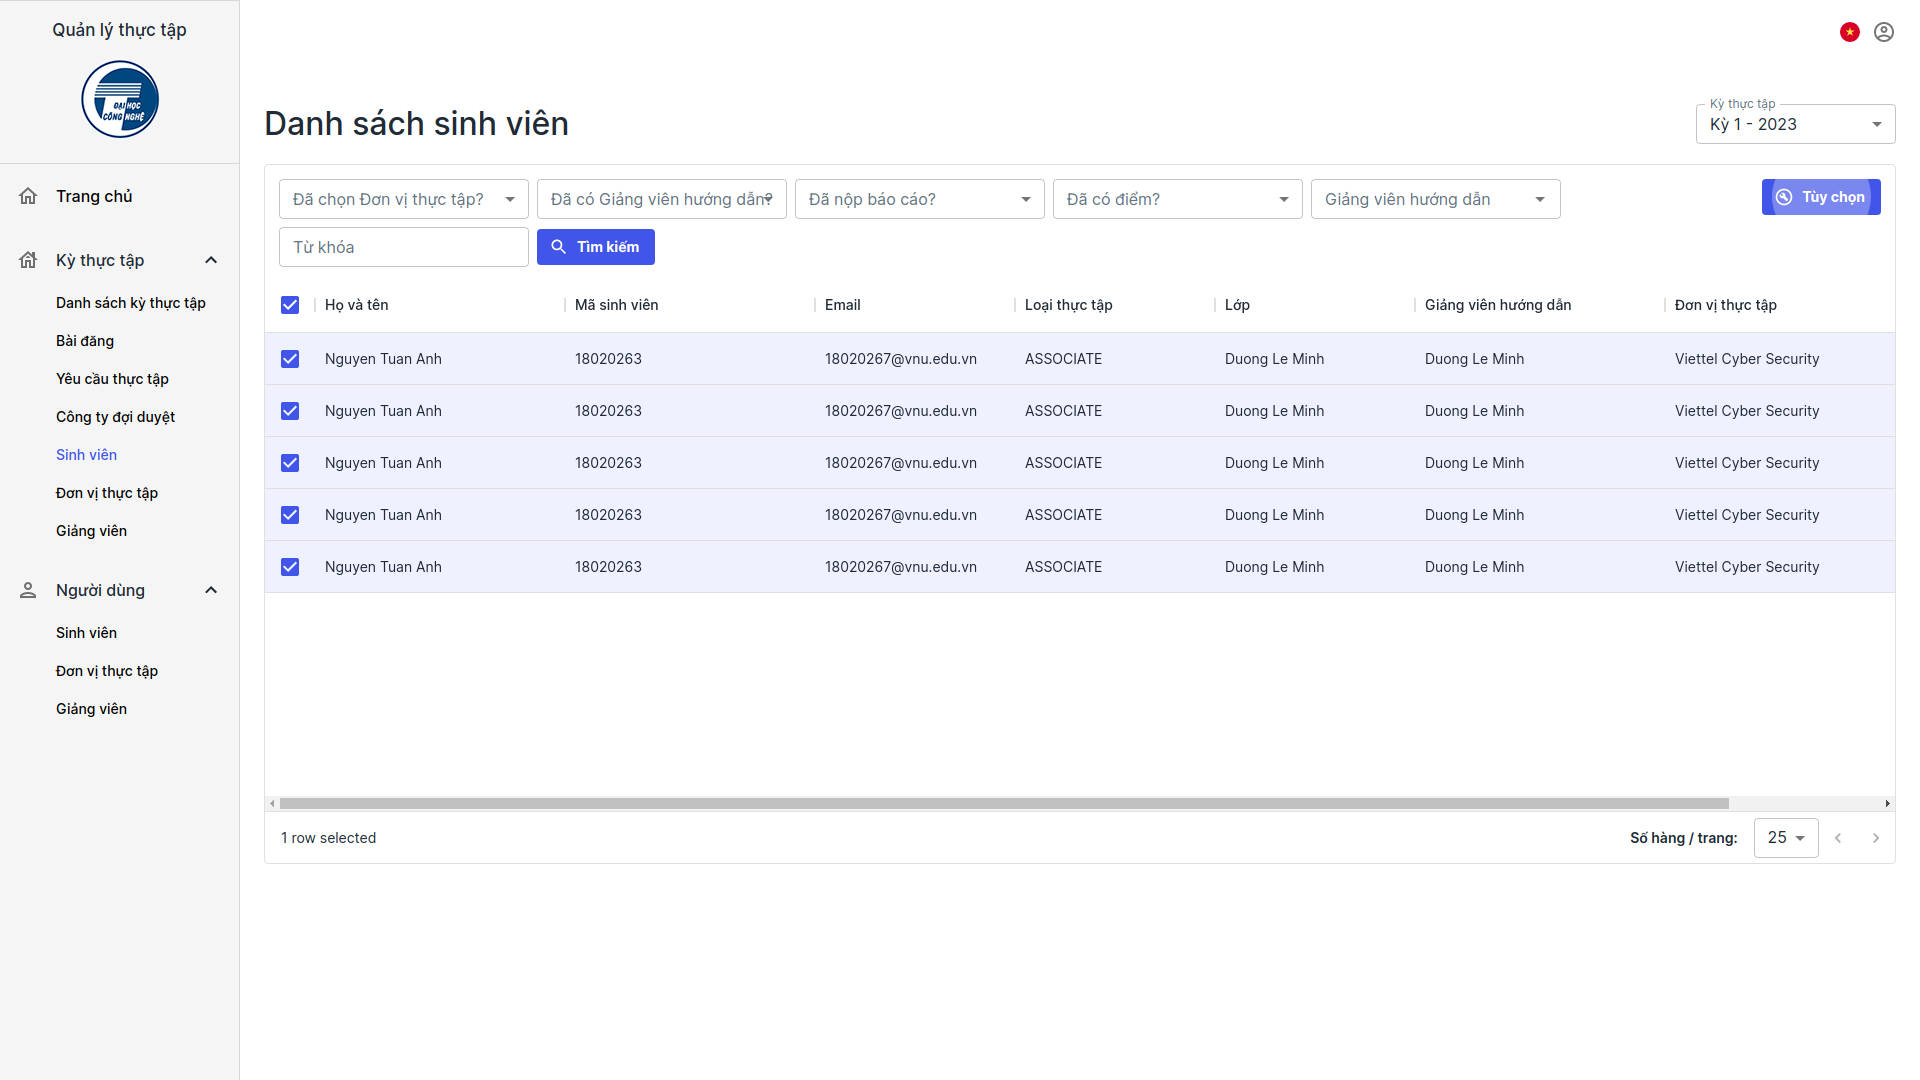
\includegraphics[width=\linewidth]{./images/image76.png}
	\caption{Luồng \emph{Quản trị viên Khoa gán giảng viên cho sinh viên}: chọn danh sách sinh viên cần gán}
	\label{fig:org_admin_select_students}
\end{figure}

\begin{figure}[]
	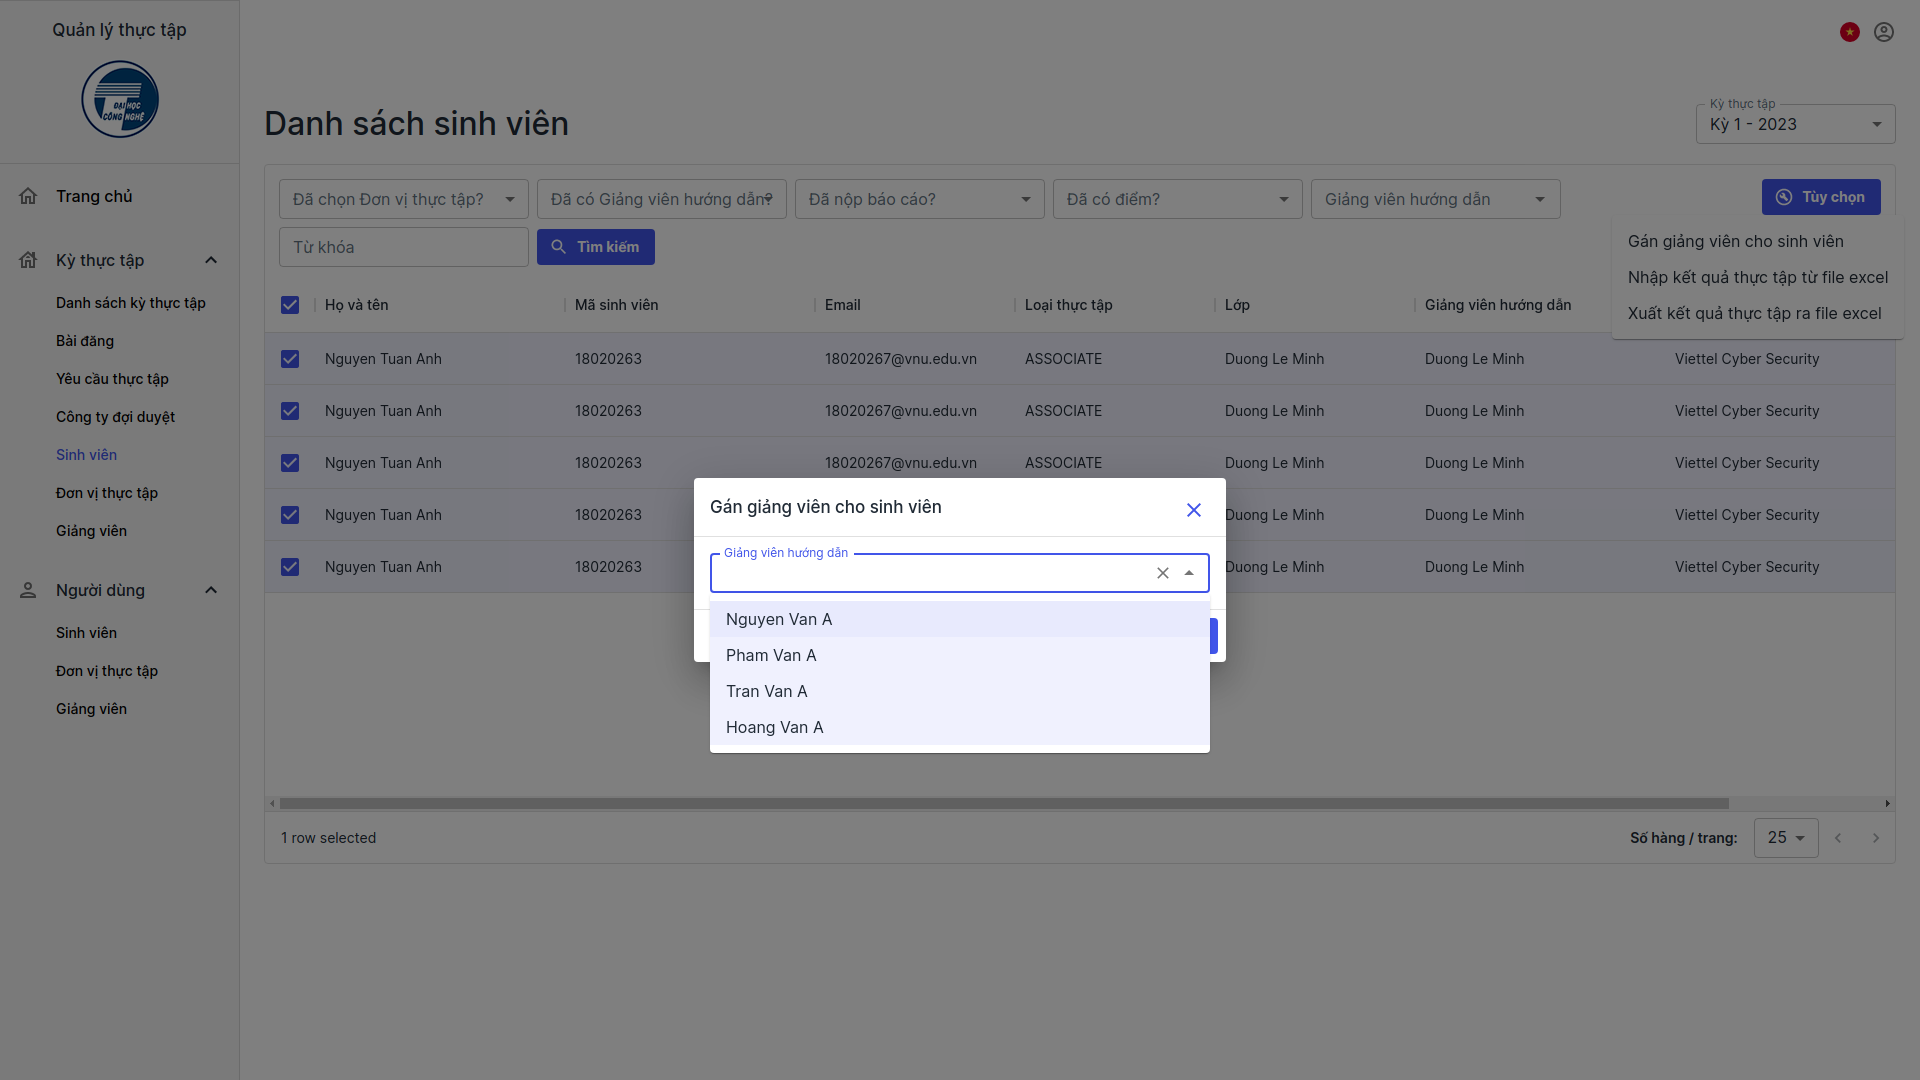
\includegraphics[width=\linewidth]{./images/image77.png}
	\caption{Luồng \emph{Quản trị viên Khoa gán giảng viên cho sinh viên}: chọn giảng viên}
	\label{fig:org_admin_select_lecturer}
\end{figure}

\begin{figure}[]
	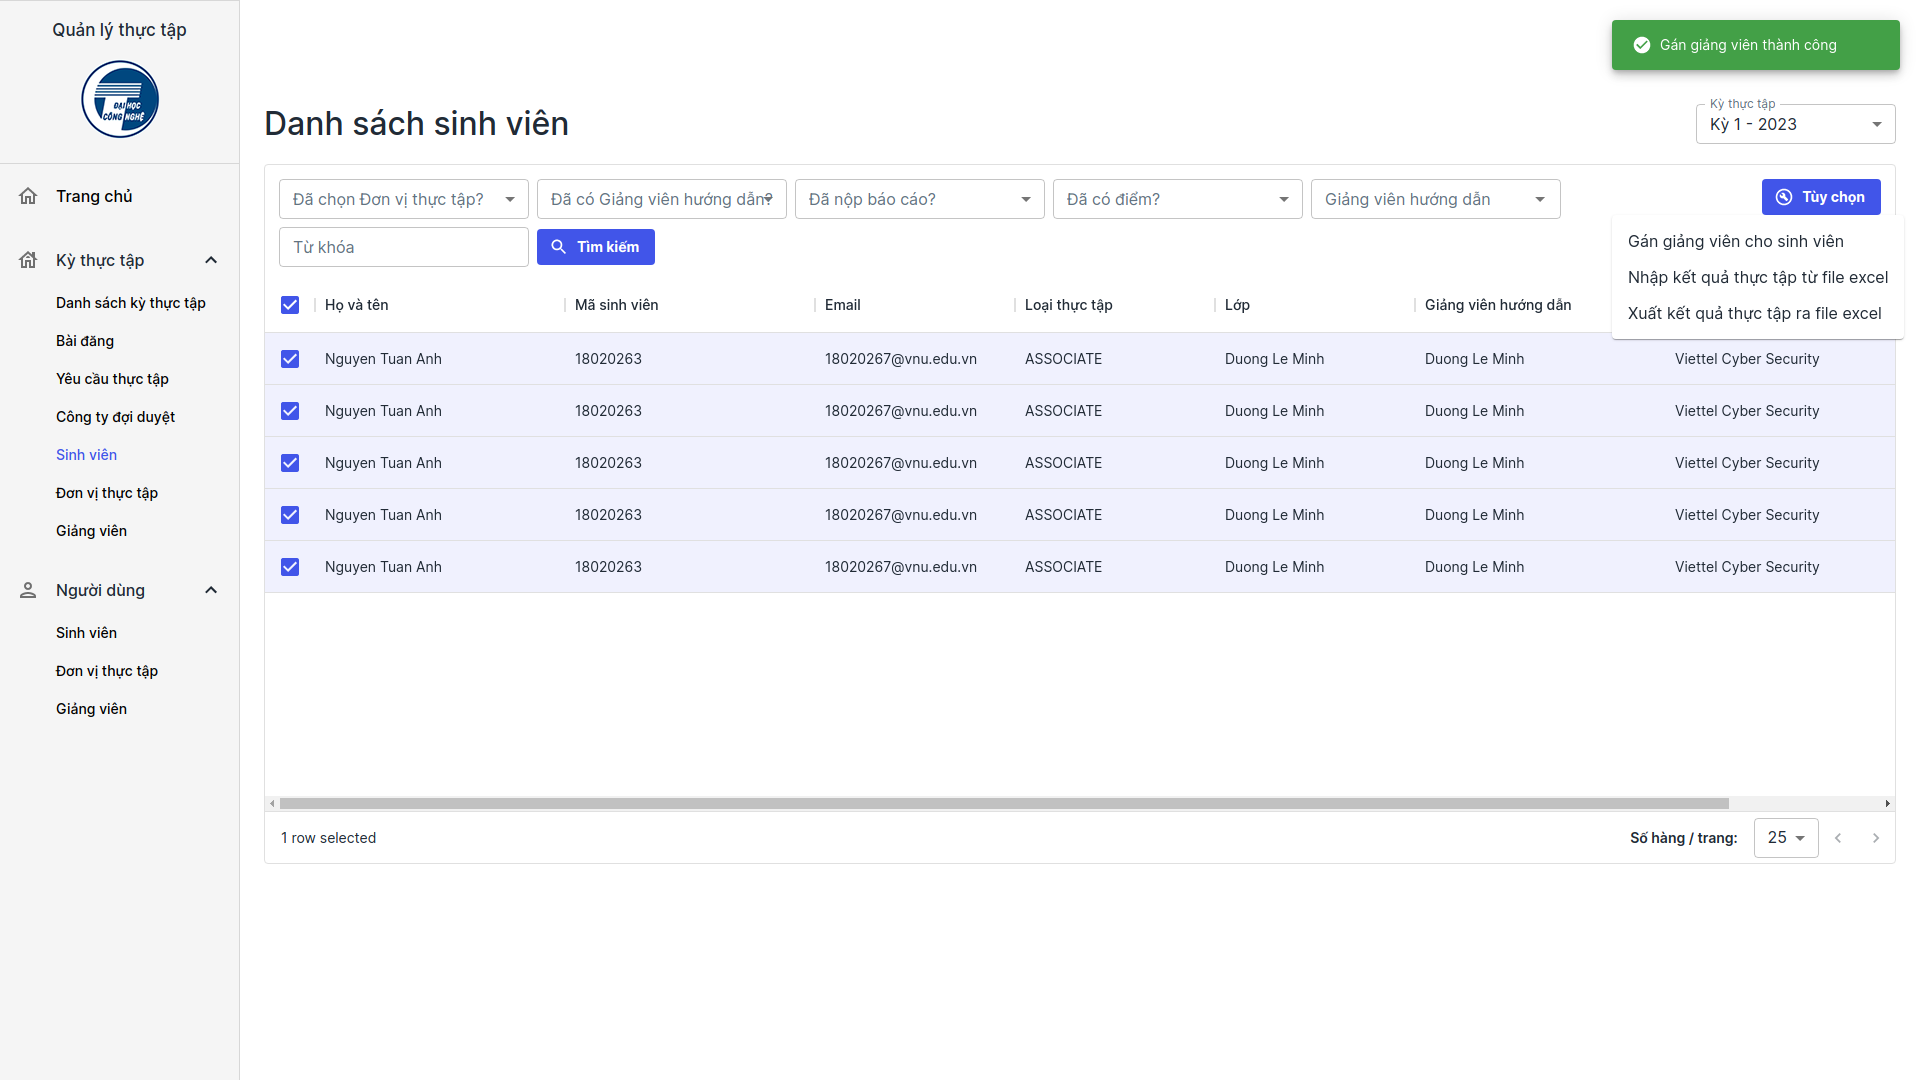
\includegraphics[width=\linewidth]{./images/image78.png}
	\caption{Luồng \emph{Quản trị viên Khoa gán giảng viên cho sinh viên}: gán giảng viên thành công}
	\label{fig:org_admin_assign_success}
\end{figure}

\paragraph*{Quản trị viên Khoa Chấp nhận / Từ chối công ty}

\begin{itemize}
	\item Hình \ref{fig:org_admin_access_list_intern_partners}: Quản trị viên truy cập danh sách Đơn vị thực tập trong kỳ thực tập và lọc ra danh sách các công ty đang ở trạng thái Pending.
	\item Hình \ref{fig:org_admin_select_partners}: Quản trị viên chọn danh sách công ty và chọn tùy chọn Chấp nhận / Từ chối công ty.
\end{itemize}

\begin{figure}[]
	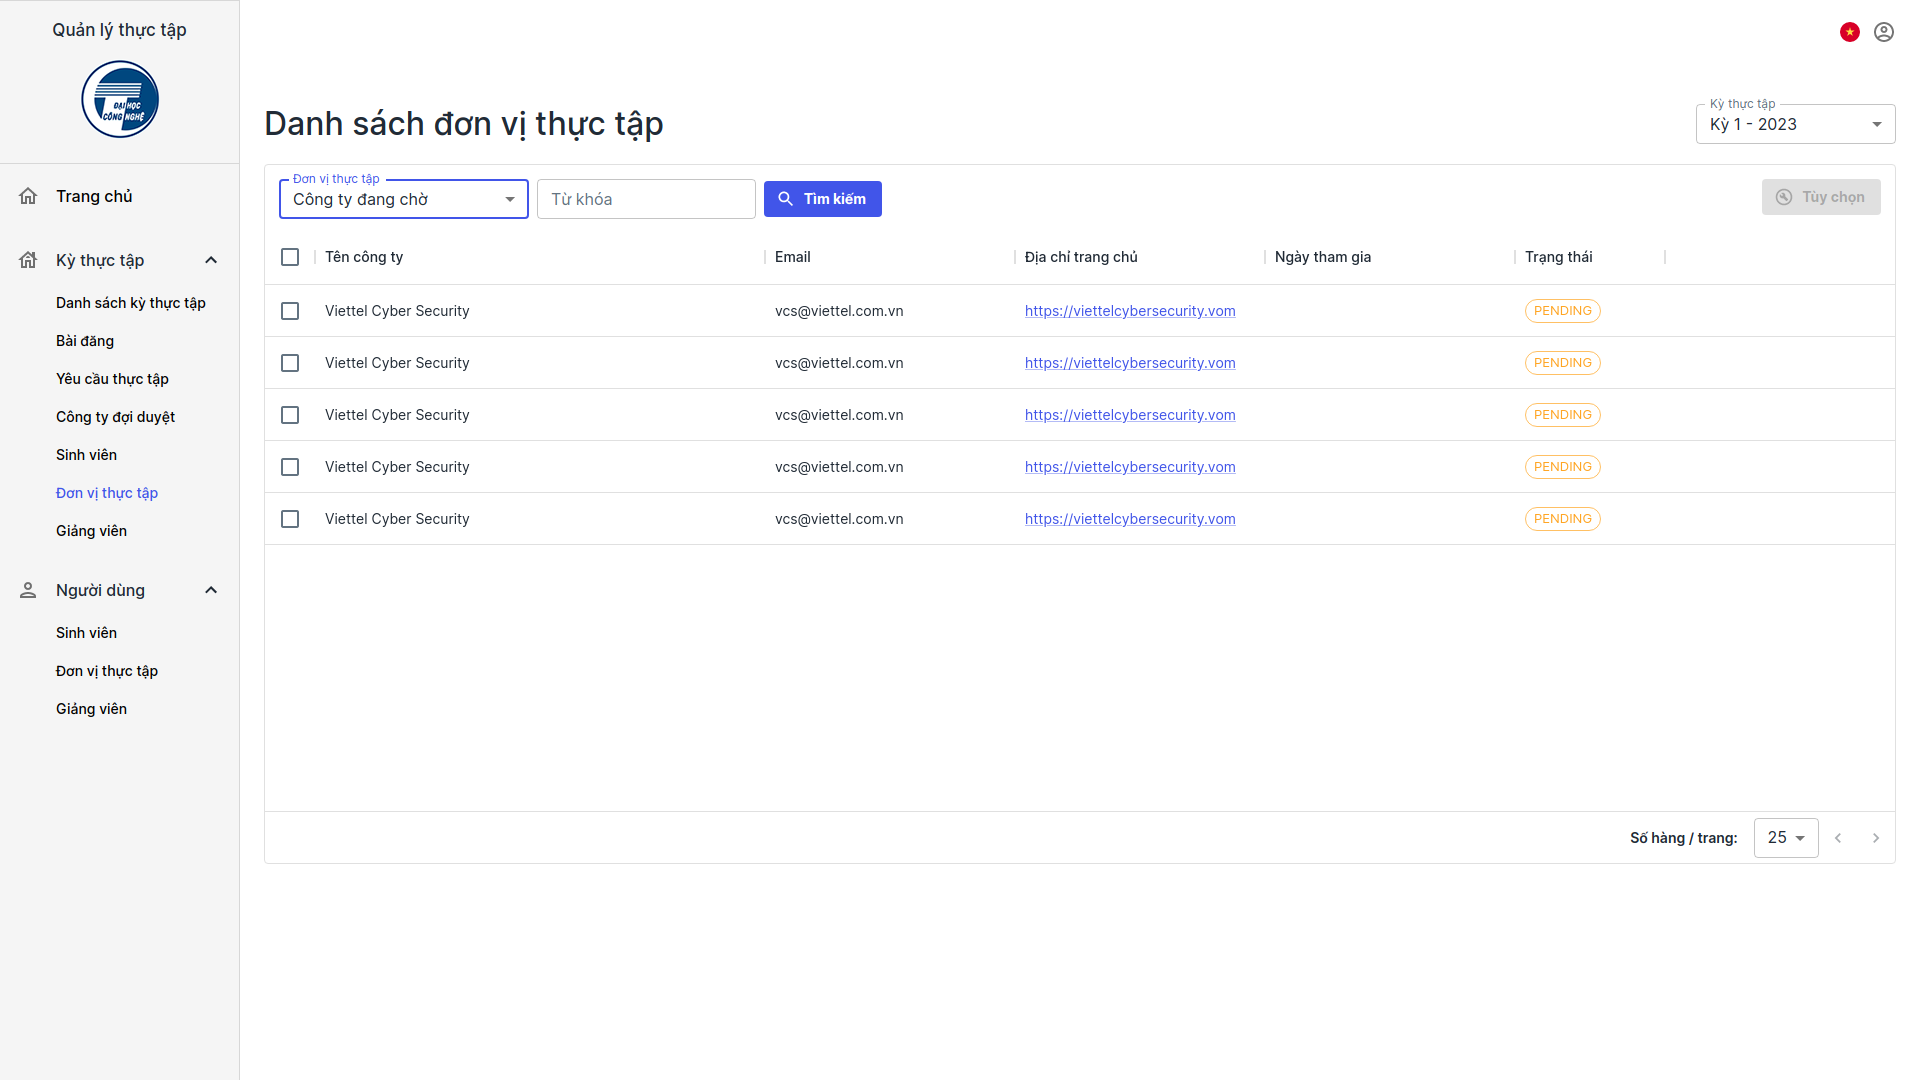
\includegraphics[width=\linewidth]{./images/image79.png}
	\caption{Luồng \emph{Quản trị viên Khoa Chấp nhận / Từ chối công ty}: truy cập danh sách đơn vị thực tập và lọc ra danh sách các công ty đang ở trạng thái Pending}
	\label{fig:org_admin_access_list_intern_partners}
\end{figure}

\begin{figure}[]
	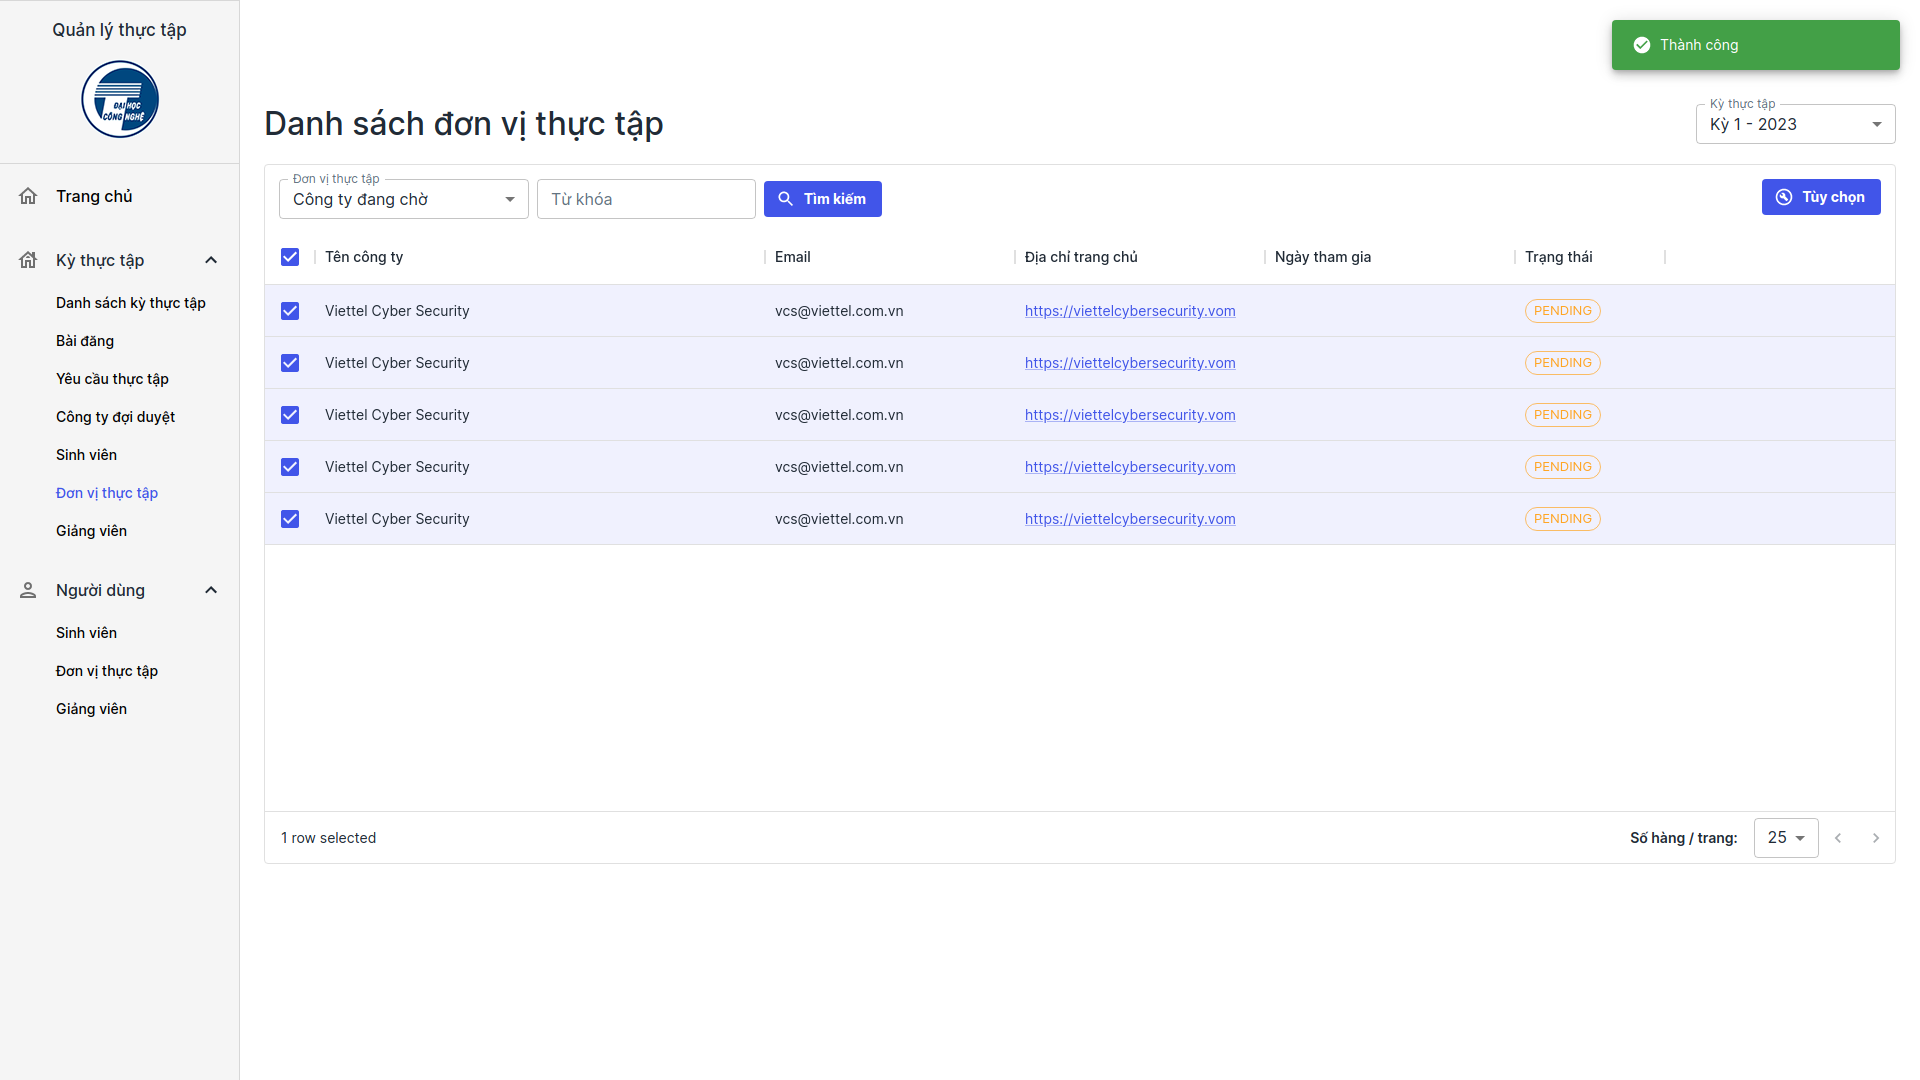
\includegraphics[width=\linewidth]{./images/image80.png}
	\caption{Luồng \emph{Quản trị viên Khoa Chấp nhận / Từ chối công ty}: chọn danh sách đơn vị thực tập và chọn tùy chọn Chấp nhận / Từ chối công ty}
	\label{fig:org_admin_select_partners}
\end{figure}

\subsubsection{Luồng sử dụng của quản trị viên hệ thống}

\paragraph*{Quản trị viên nhập vào Danh sách sinh viên}

\begin{itemize}
	\item Hình \ref{fig:admin_access_list_students}: Quản trị viên truy cập danh sách sinh viên và mở tùy chọn.
	\item Hình \ref{fig:choose_file}: Quản trị viên chọn Nhập danh sách sinh viên từ file excel và chọn tệp.
	\item Hình \ref{fig:upload_list}: Quản trị viên duyệt qua danh sách sau khi chọn tệp và tải lên danh sách.
\end{itemize}

\begin{figure}[]
	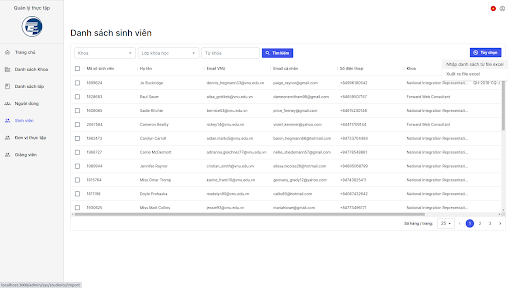
\includegraphics[width=\linewidth]{./images/image68.png}
	\caption{Luồng \emph{Quản trị viên nhập vào Danh sách sinh viên}: truy cập danh sách sinh viên và mở tùy chọn}
	\label{fig:admin_access_list_students}
\end{figure}

\begin{figure}[]
	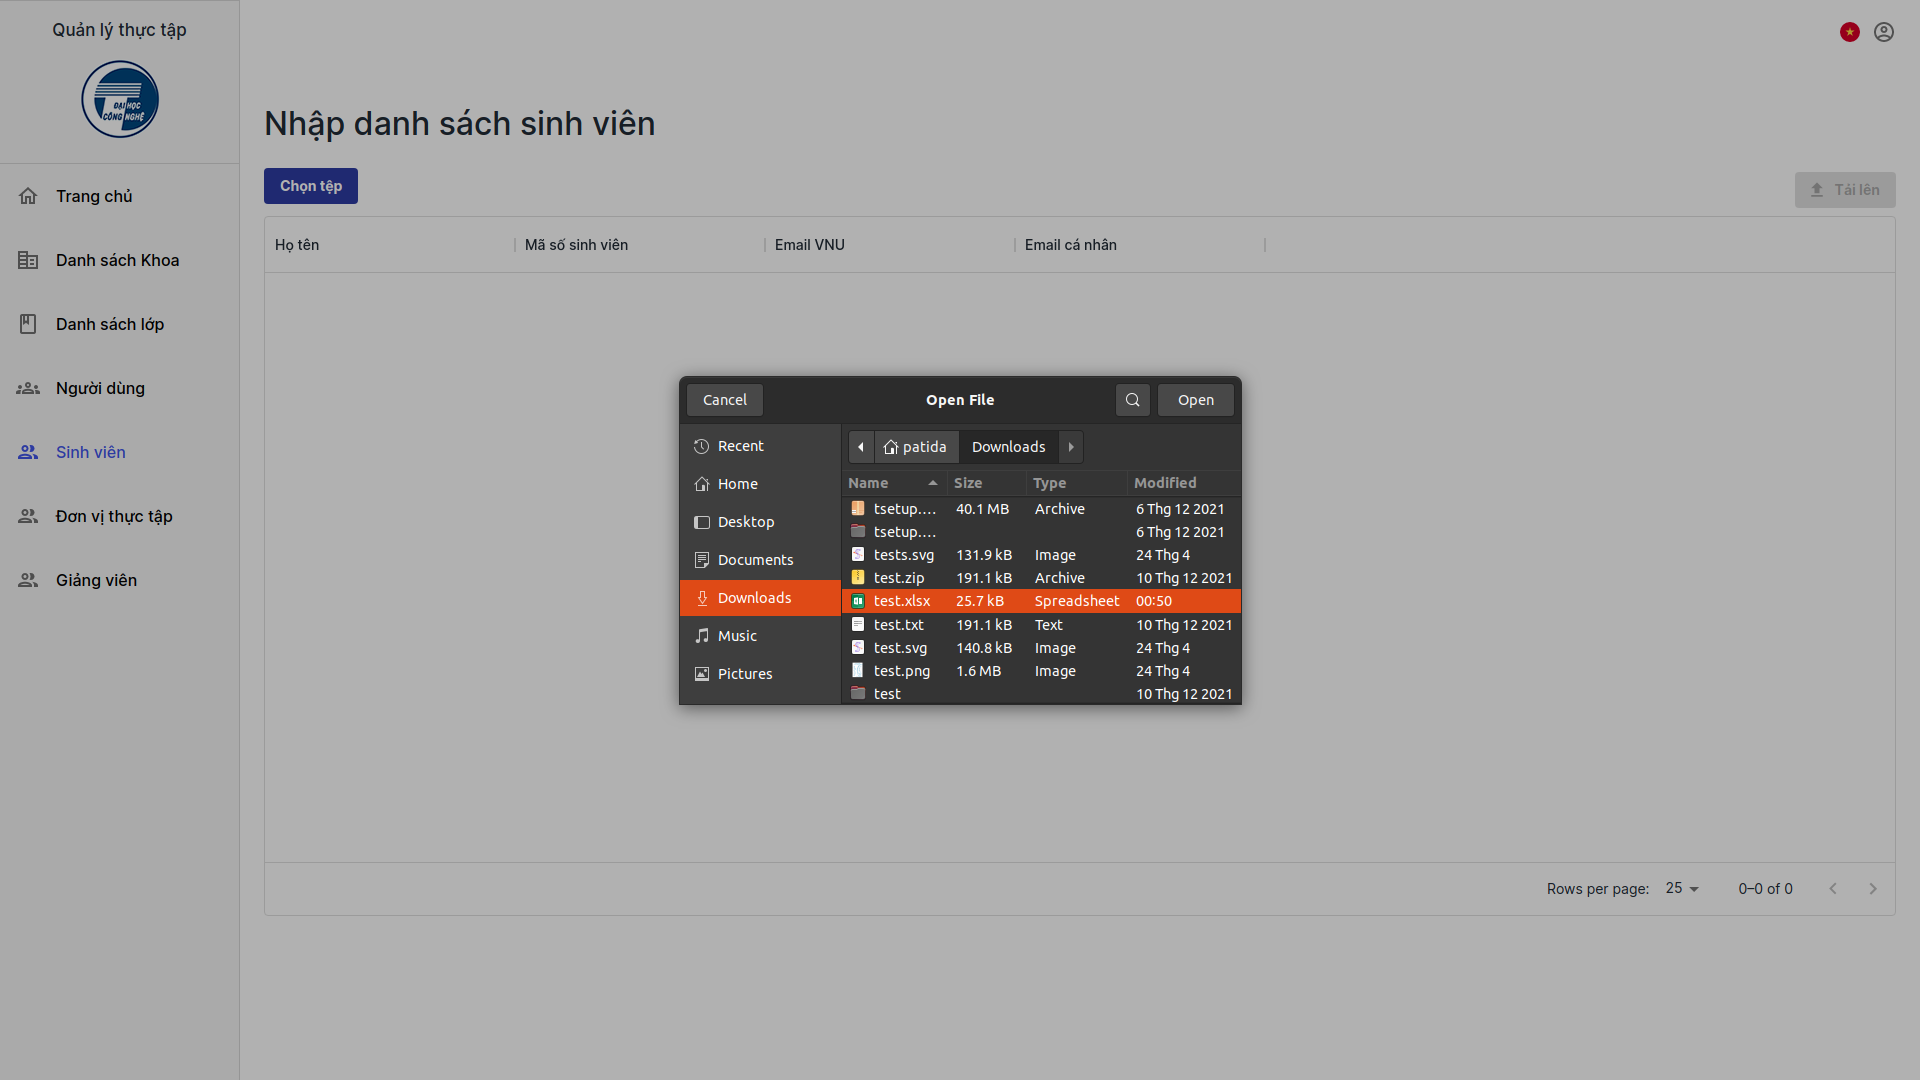
\includegraphics[width=\linewidth]{./images/image27.png}
	\caption{Luồng \emph{Quản trị viên nhập vào Danh sách sinh viên}: chọn Nhập danh sách sinh viên từ file excel và chọn tệp danh sách sinh viên}
	\label{fig:choose_file}
\end{figure}

\begin{figure}[]
	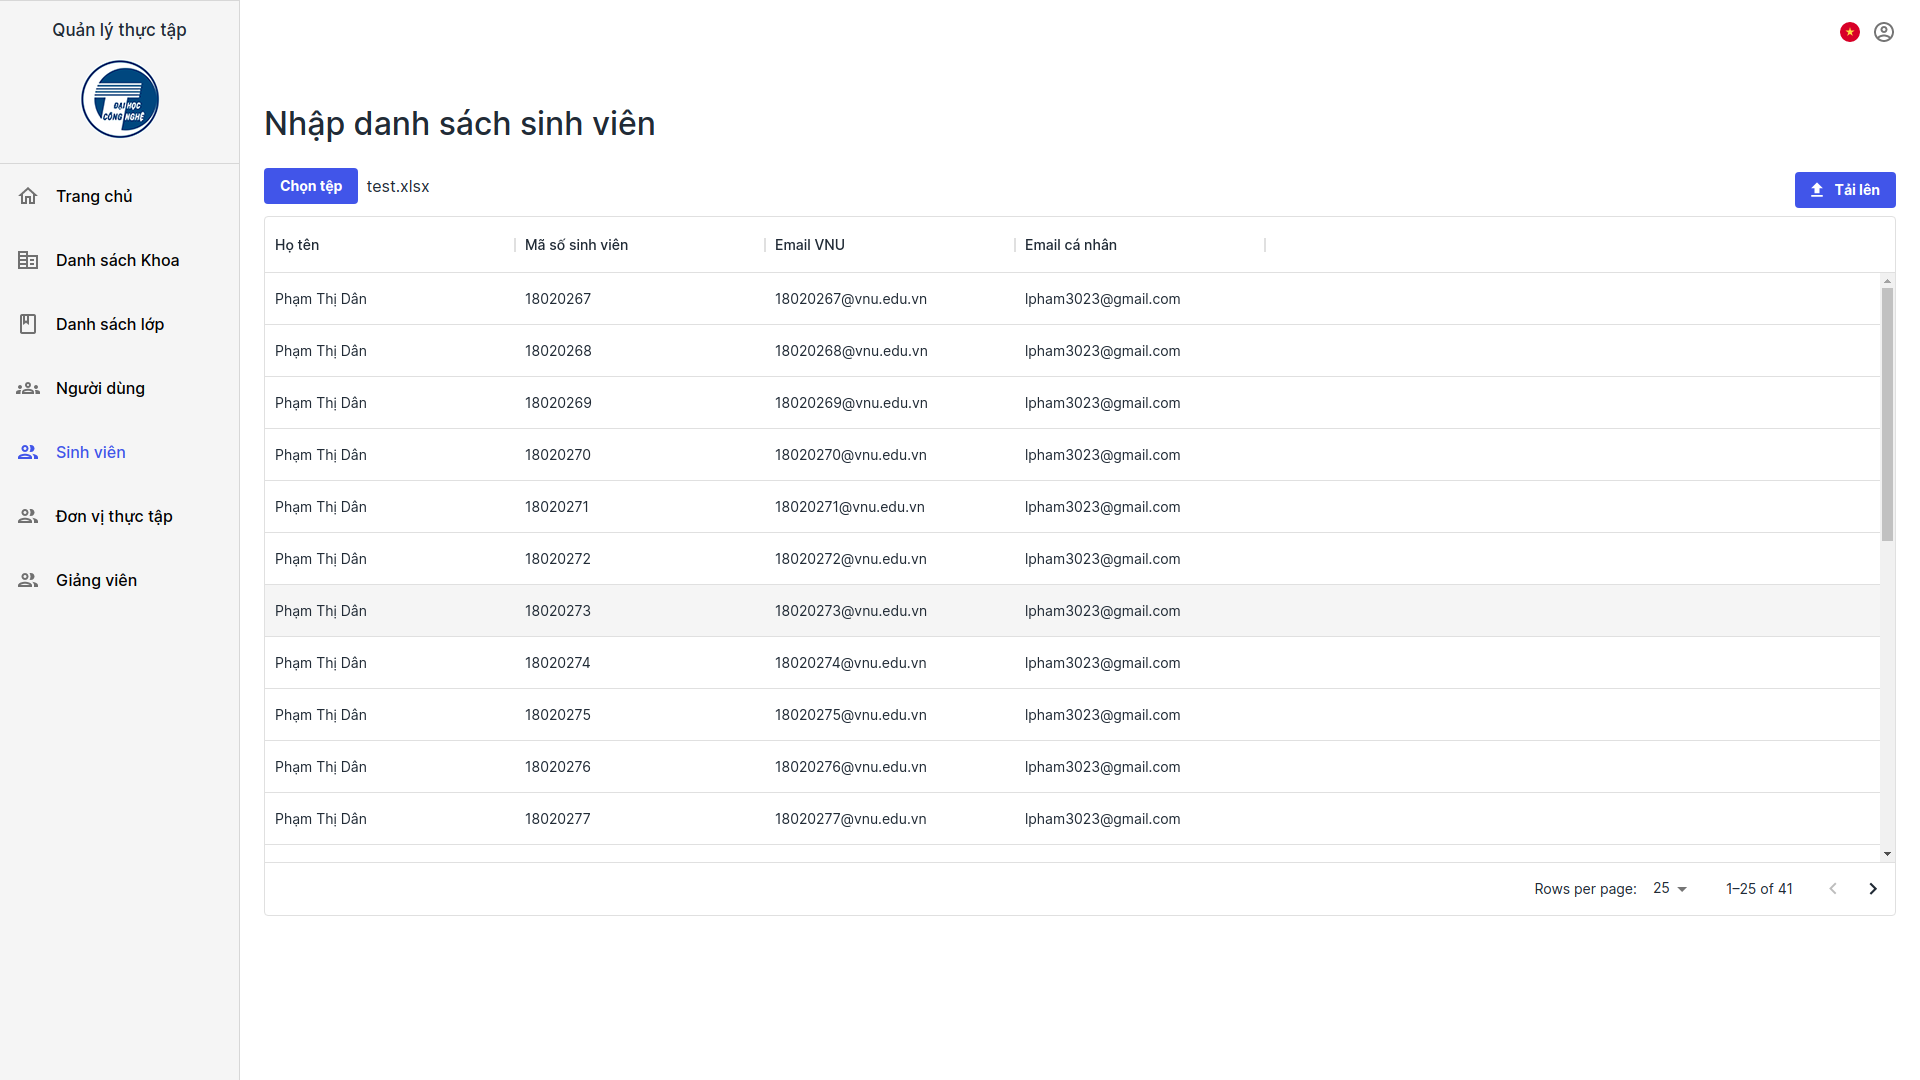
\includegraphics[width=\linewidth]{./images/image28.png}
	\caption{Luồng \emph{Quản trị viên nhập vào Danh sách sinh viên}: duyệt qua danh sách sau khi chọn tệp và tải lên danh sách}
	\label{fig:upload_list}
\end{figure}

\paragraph*{Quản trị viên đặt lại mật khẩu cho người dùng}

\begin{itemize}
	\item Hình \ref{fig:admin_access_list_users}: Quản trị viên truy cập danh sách Người dùng và chọn Đặt lại mật khẩu.
	\item Hình \ref{fig:reset_password_success}: Đặt lại mật khẩu thành công.
\end{itemize}

\begin{figure}[]
	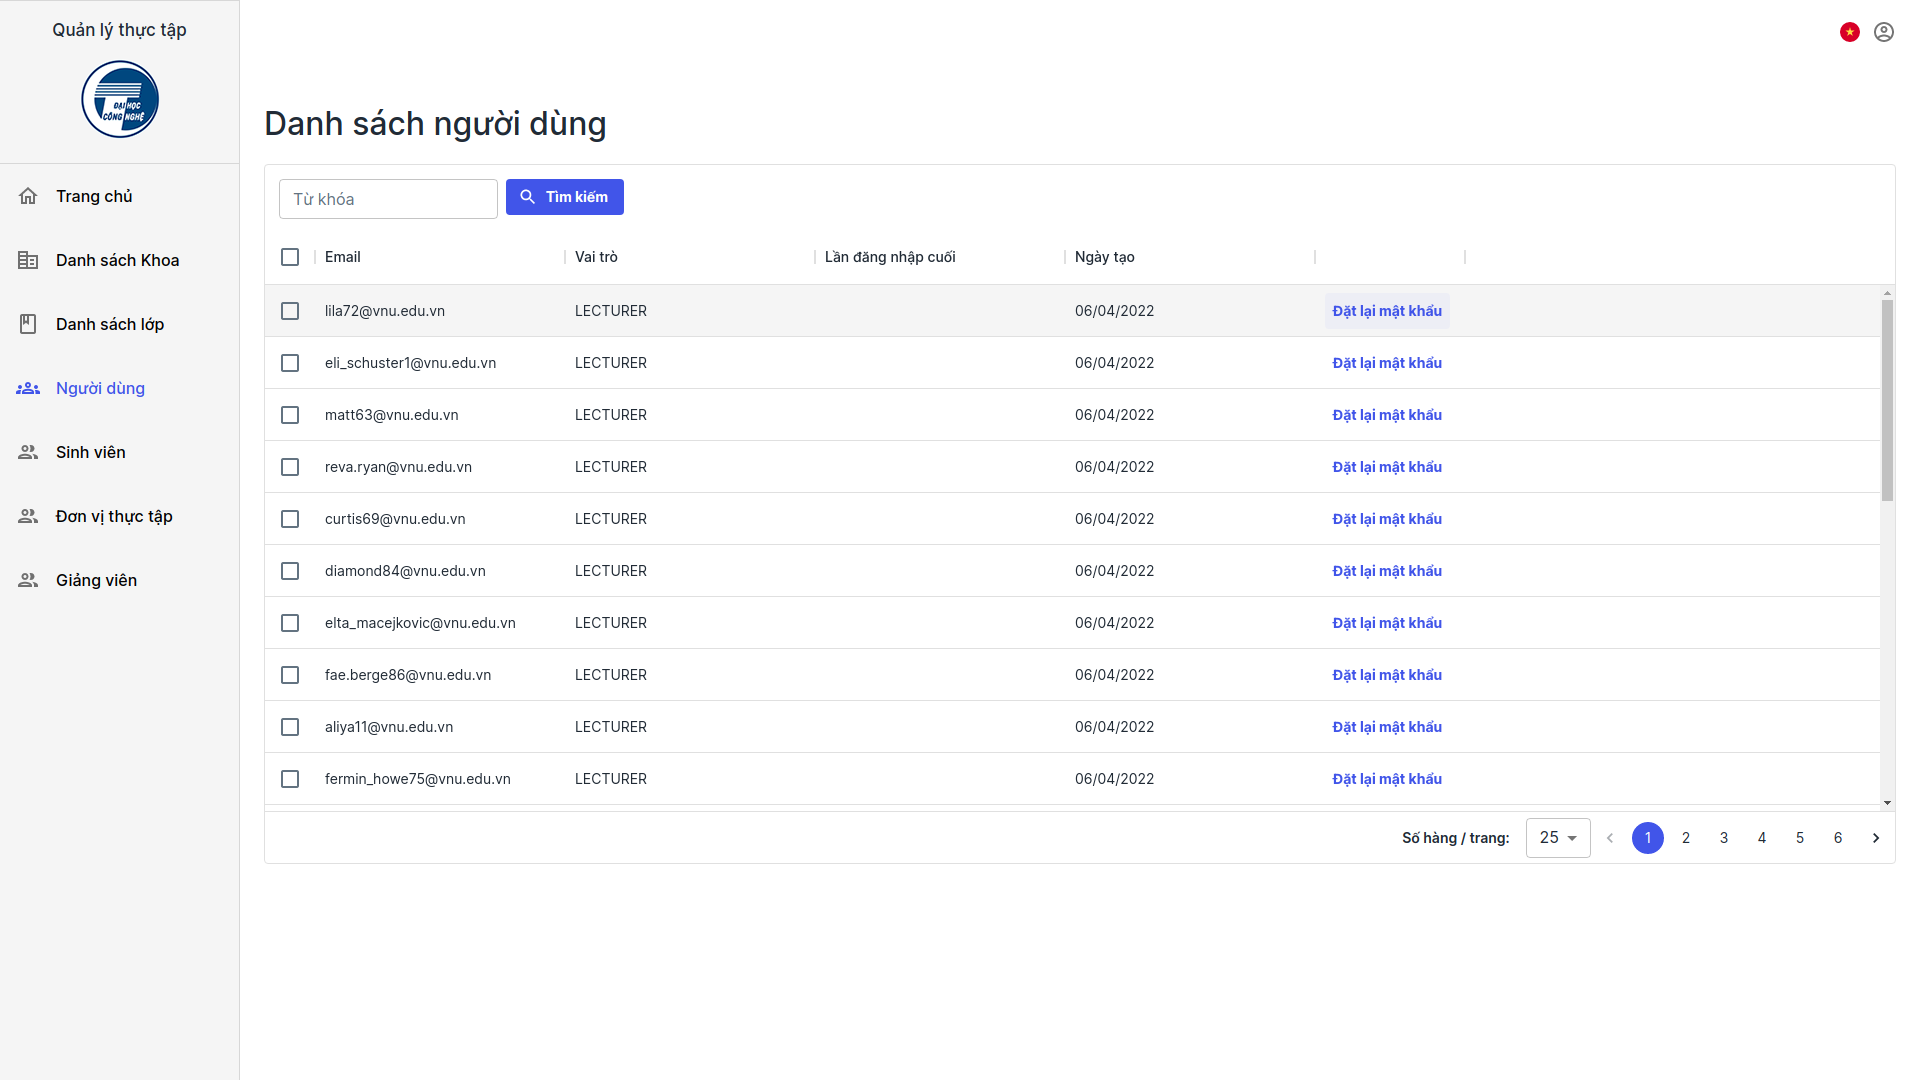
\includegraphics[width=\linewidth]{./images/image69.png}
	\caption{Luồng \emph{Quản trị viên đặt lại mật khẩu cho người dùng}: truy cập danh sách Người dùng và chọn Đặt lại mật khẩu}
	\label{fig:admin_access_list_users}
\end{figure}

\begin{figure}[]
	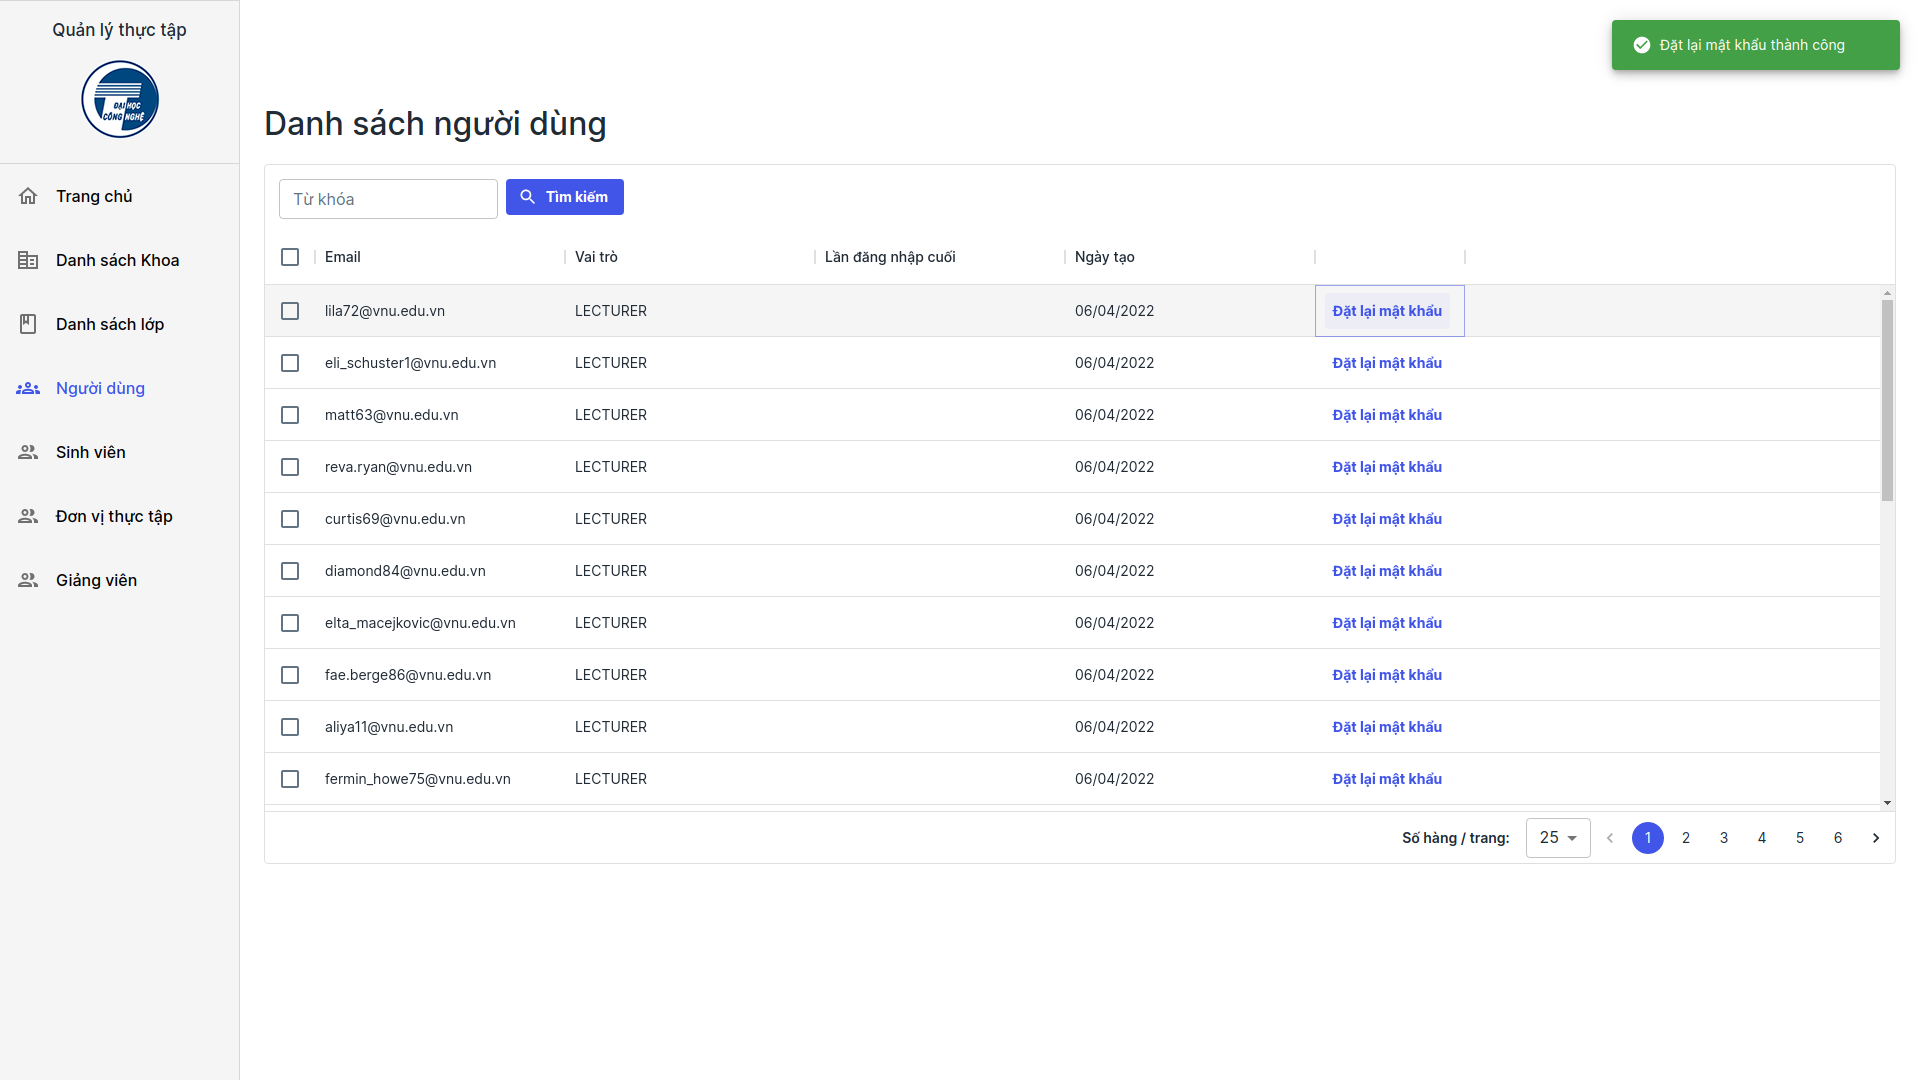
\includegraphics[width=\linewidth]{./images/image70.png}
	\caption{Luồng \emph{Quản trị viên đặt lại mật khẩu cho người dùng}: Đặt lại mật khẩu thành công}
	\label{fig:reset_password_success}
\end{figure}

\end{document}